%%%%%%%%%%%%%%%%%%%%%%%%%%%%%%%%%%%%%%%%%%%%%%%%%%%%%%%%%%%%%%%%%%%%%
% In English:
%    This is a Latex template for São Paulo Research Foudation (FAPESP)
%         reports (annual or final).
%    This is the modified version of the original Latex template from
%         following website.
%    Original Source: http://www.howtotex.com
%    For information about FAPESP, check http://www.fapesp.br/en
%    This template targets mainly on reports in Portuguese language.
%    New additions and changes in the latest version:
%        - Added the possibility of including multiple members in the
%          research team, with the commands \memberA{Name of Member A}
%          \memberB{Name of Member B} \memberC{Name of Member C} etc.
%        - Included commands to define project modality and the research
%          agency (if you want to use the same model for other research
%          agencies such as CAPES, CNPq etc).
%
% In Portuguese:
%    Este é um modelo Latex para relatórios (anual ou final) da Fundação
%         de Amparo à pesquisa do Estado de São Paulo (FAPESP).
%    Esta é uma versão modificada do modelo Latex do site supra mencionado.
%    Para informações sobre a FAPESP, verifique http://www.fapesp.br
%    Esse modelo foca principalmente nos relatórios escritos em Português.
%    Novas adições e alterações na última versão:
%       - Foi adicionada a possibilidade de incluir vários membros no
%         grupo de pesquisas, com os comandos \membroA{Nome do Membro A}
%         \membroB{} \membroC{} etc.
%       - Foram incluídos comandos para definir modalidade de projeto e
%         agência de fomento (caso queira utilizar o mesmo modelo para
%         outras agências, CAPES, CNPq etc).
%
% Author/Autor: André Leon Sampaio Gradvohl, Dr.
% Email:        andre.gradvohl@gmail.com
% Lattes CV:    http://lattes.cnpq.br/9343261628675642
% GitHub: http://gradvohl.github.io/
%
% Last update/Última versão: 19/Feb/2018
%
%%%%%%%%%%%%%%%%%%%%%%%%%%%%%%%%%%%%%%%%%%%%%%%%%%%%%%%%%%%%%%%%%%%%%%
\documentclass[12pt]{report}
\usepackage[a4paper]{geometry}
\usepackage[utf8]{inputenc}
\usepackage[english,portuguese]{babel}
\usepackage[myheadings]{fullpage}
\usepackage[T1]{fontenc}
\usepackage{fancyhdr}
\usepackage{setspace}
\usepackage{sectsty}
\usepackage{url}

%%% iniciar capitulo na mesma pagina (Mateus) %%%
\usepackage{etoolbox}
\makeatletter %inicio da modificacao (iniciar capitulo na msma pag)
\patchcmd{\chapter}{\if@openright\cleardoublepage\else\clearpage\fi}{}{}{}
\makeatother %fim da modificacao
%%% iniciar capitulo na mesma pagina (Mateus) %%%

%%------
%% Comandos gerais
%% Observação: o arquivo "comandos.tex" tem que estar presente.
%%------
%%%%%%%%%%%%%%%%%%%%%%%%%%%%%%%%%%%%%%%%%%%%%%%%%%%%%%%%%%%%%%%%%%%%%
% In English:
%    This is a list of commands specification for FAPESP reports.
%
% In Portuguese:
%    Esta é uma lista de especificação de comandos para relatórios
% da Fundação de Amparo à pesquisa do Estado de São Paulo (FAPESP).
%
% Author/Autor: André Leon Sampaio Gradvohl, Dr.
% Email:        andre.gradvohl@gmail.com
% Lattes CV:    http://lattes.cnpq.br/9343261628675642
%
% Last update/Última versão: 11/Sep/2016
%%%%%%%%%%%%%%%%%%%%%%%%%%%%%%%%%%%%%%%%%%%%%%%%%%%%%%%%%%%%%%%%%%%%%%

\newcommand{\HRule}[1]{\rule{\linewidth}{#1}}
\setcounter{tocdepth}{3}
\setcounter{secnumdepth}{3}

\newcommand{\titulo}[1]{\def\meuTitulo{#1}}
\newcommand{\tituloIngles}[1]{\def\meuTituloIngles{#1}}
\newcommand{\numProjeto}[1]{\def\numFAP{#1}}
\newcommand{\tipoRelatorio}[1]{\def\tipoRelat{#1 }} %o espaço depois do #1 é importante
\newcommand{\modalidadeProjeto}[1]{\def\modProjeto{#1}}
\newcommand{\agFomento}[2]{\def\agFom{#1} \def\siglaAgFom{#2}} %extenso Sigla
\newcommand{\autor}[1]{\def\nomeAutor{#1}}
\newcommand{\cidade}[1]{\def\nomeCidade{#1}}
\newcommand{\universidade}[1]{\def\nomeUniversidade{#1}}
\newcommand{\faculdade}[1]{\def\nomeFaculdade{#1}}
\newcommand{\periodoVigencia}[1]{\def\periodVig{#1}}
\newcommand{\periodoRelatorio}[1]{\def\periodRelat{#1}}
\newcommand{\orientador}[1]{\def\nomeOrientador{#1}}

\newcommand\namegroup[2]{%
   \begin{minipage}[t]{0.4\textwidth}
   \hspace{0.6cm}
   \begin{tikzpicture}
   \node[anchor=south east,inner sep = 0](signF){\includegraphics[width=5cm]{#2}};
   \end{tikzpicture}
   \vspace*{0.1cm}  % leave some space above the horizontal line
   \hrule
   \vspace{1mm} % just a bit more whitespace below the line
   \centering
   \begin{tabular}[t]{c}
   #1
   \end{tabular}
   \end{minipage}}

\author{}
\date{}

%Definição de membros da equipe de pesquisas
\newcommand{\membroA}[1]{\def\nomeMembroA{#1}}
\newcommand{\membroB}[1]{\def\nomeMembroB{#1}}
\newcommand{\membroC}[1]{\def\nomeMembroC{#1}}
\newcommand{\membroD}[1]{\def\nomeMembroD{#1}}
\newcommand{\membroE}[1]{\def\nomeMembroE{#1}}
\newcommand{\membroF}[1]{\def\nomeMembroF{#1}}

\newcommand{\Figure}[1]{Figura~\ref{fig:#1}}
\newcommand{\Table}[1] {Tabela~\ref{#1}}
\newcommand{\Equation}[1] {Equa\c{c}\~ao~\ref{#1}}
\newcommand{\addFigure}[3] { %Parametros scale, fig_name, caption
    \begin{figure}[!hbt]
      \centering
      \includegraphics[scale=#1]{figures/}
      \caption{#3}\label{fig:#2}
    \end{figure}
}

\newcommand{\geraTitulo}{
\clearpage
\begin{titlepage}
  \begin{center}
      \vspace*{-3cm}
       { \setstretch{.5}
         \textsc{\nomeUniversidade} \\
         \HRule{.2pt}\\
         \textsc{\nomeFaculdade}
       }

       \vspace{5.5cm}

       \Large \textbf{\textsc{\meuTitulo}}
 	  \HRule{1.5pt} \\ [0.5cm]
       \linespread{1}
       \large Relatório Científico
       \ifdefined\tipoRelat
            \tipoRelat
       \fi
       do projeto
       \ifdefined\modProjeto
           na modalidade \modProjeto,
       \fi
       fomentado pela \agFom. \\
   	   \HRule{1.5pt} \\ [0.5cm]

       \ifdefined\numFAP
          Projeto \siglaAgFom~\texttt{\#\numFAP}
          \\ [0.5cm]
       \fi
        Aluno: \nomeAutor \\
        Orientadora: \nomeOrientador \\[5.cm]

        % aqui começa a adicao das linhas de assinatura
        %Aluno: \tikz\draw [thick,solid] (0,0) -- (6,0); \\[.5cm]
        %Orientador: \tikz\draw [thick,solid] (0,0) -- (5.5,0);


        \namegroup{Aluno}{fig/assinatura-mateus.png}
        \hspace{1.5cm}
        \namegroup{Orientadora}{fig/assinatura-funchal.png}

        %\begin{minipage}[t]{0.4\textwidth}
        %\vspace*{1.5cm}
        %\hrule
        %\vspace{1mm}
        %\centering
        %\begin{tabular}[t]{c}
        %Aluno
        %\end{tabular}
        %\hspace{1.5cm}
        %\begin{minipage}[t]{0.4\textwidth}
        %\vspace*{1.5cm}
        %\hrule
        %\vspace{1mm}
        %\centering
        %\begin{tabular}[t]{c}
        %Aluno
        %\end{tabular}
        %\end{minipage}
        %%\hfill

        \vfill

        {\normalsize  \nomeCidade, \today}
 \end{center}
 \end{titlepage}
}

\usepackage{titlesec}
\titleformat{\chapter}{\normalfont\LARGE\bfseries}{\thechapter}{1em}{}
\titlespacing*{\chapter}{0pt}{3.5ex plus 1ex minus .2ex}{2.3ex plus .2ex}

%----------------------------------------------------------------------
% Cabeçalho e rodapé
%----------------------------------------------------------------------
\pagestyle{fancy}
\fancyhf{} % Limpa todos os campos de header and footer fields
\renewcommand{\headrulewidth}{0pt}
\fancyfoot[R]{\thepage}

\addto\captionsportuguese{\renewcommand{\contentsname}{Sumário}}
\addto\captionsportuguese{\renewcommand{\bibname}{Referências Bibliográficas}}

%------
% Resumo e Abstract
%------
\newcommand{\Resumo}[1]{
   \begin{otherlanguage}{portuguese}
       \addcontentsline{toc}{chapter}{Resumo}
       \begin{abstract} \thispagestyle{plain} \setcounter{page}{2}
          #1
        \end{abstract}
   \end{otherlanguage}
} %end \Resumo

\newcommand{\Abstract}[1]{
   \begin{otherlanguage}{english}
      \addcontentsline{toc}{chapter}{Abstract}
      \begin{abstract} \thispagestyle{plain} \setcounter{page}{3}
       #1
      \end{abstract}
    \end{otherlanguage}
} %end \abstract

%------
% Folha de rosto
%------
\newcommand{\folhaDeRosto}{
   \chapter*{Informações Gerais do Projeto}
   \addcontentsline{toc}{chapter}{Informações Gerais do Projeto}
   \begin{itemize}
      \item Título do projeto:
            \begin{itemize}\item[] \textbf{\meuTitulo} \end{itemize}
      \item Nome do pesquisador responsável:
            \begin{itemize}\item[]\textbf{Profa. \nomeOrientador}\end{itemize}
      \item Instituição sede do projeto:
            \begin{itemize}
               \item[]\textbf{\nomeFaculdade \ da \nomeUniversidade}
            \end{itemize}
      \item Equipe de pesquisa:
            \begin{itemize}
               \ifdefined\nomeMembroA
                 \item[]\textbf{\nomeMembroA}
               \else
                 \item[]\textbf{\nomeAutor}
               \fi
               \ifx\nomeMembroB\undefined\else \item[]\textbf{\nomeMembroB}\fi
               \ifx\nomeMembroC\undefined\else \item[]\textbf{\nomeMembroC}\fi
               \ifx\nomeMembroD\undefined\else \item[]\textbf{\nomeMembroD}\fi
               \ifx\nomeMembroE\undefined\else \item[]\textbf{\nomeMembroE}\fi
               \ifx\nomeMembroF\undefined\else \item[]\textbf{\nomeMembroF}\fi
             \end{itemize}

          \ifdefined \numFAP
             \item Número do projeto de pesquisa:
             \begin{itemize}
                 \item[]\textbf{\numFAP}
             \end{itemize}
          \fi
       \item Período de vigência:
            \begin{itemize}
               \item[]\textbf{\periodVig}
            \end{itemize}
       \item Período coberto por este relatório científico:
            \begin{itemize}
               \item[]\textbf{\periodRelat}
            \end{itemize}
   \end{itemize}
   \clearpage
}

\usepackage{mathtools}
%\usepackage{amsthm}
\usepackage{amsmath}
%\usepackage{nccmath}
\usepackage{amssymb}
%\usepackage{amsfonts}
\usepackage{physics}
%\usepackage{dsfont}
%\usepackage{mathrsfs}
%\usepackage{slashed}    % Feynman slash notation, requires LuaLaTeX
%\usepackage[compat=1.1.0]{tikz-feynman}   % Feynman diagrams

%\usepackage{titling}
\usepackage{indentfirst}
%\usepackage[titletoc,title]{appendix}
%\renewcommand\appendixname{Apêndice}

\usepackage{bm}
%\usepackage{xcolor}
%\usepackage[dvipsnames]{xcolor}
\usepackage{cancel}

%\usepackage{xurl}
\usepackage{hyperref}
\usepackage{cite}

\usepackage{float}
\usepackage{graphicx}
\usepackage{tikz}
\usepackage{caption}
\usepackage{subcaption}

%%%%%%%%%%%%%%%%%%%%%%%%%%%%%%%%%%%%%%%%%%%%%%%%%%%

\newcommand{\eps}{\epsilon}
\newcommand{\vphi}{\varphi}
\newcommand{\cte}{\text{cte}}

\newcommand{\N}{\mathbb{N}}
\newcommand{\Z}{\mathbb{Z}}
\newcommand{\Q}{\mathbb{Q}}
\newcommand{\R}{\mathbb{R}}
\newcommand{\C}{\mathbb{C}}
\renewcommand{\P}{\mathbb{P}}
\renewcommand{\H}{\s{H}}

\newcommand{\0}{\vb{0}}
\newcommand{\1}{\mathds{1}}
\newcommand{\E}{\vb{E}}
\newcommand{\B}{\vb{B}}
\renewcommand{\v}{\vb{v}}
\renewcommand{\r}{\vb{r}}
\newcommand{\p}{\vb{p}}
\newcommand{\q}{\vb{q}}
\newcommand{\F}{\vb{F}}
\newcommand{\dtcp}{\delta_{\text{CP}}}

\newcommand{\s}[1]{\mathcal{#1}}
\renewcommand{\sl}[1]{\slashed{#1}}
\newcommand{\prodint}[2]{\left\langle #1 , #2 \right\rangle}
\newcommand{\cc}[1]{\overline{#1}}
\newcommand{\Eval}[3]{\eval{\left( #1 \right)}_{#2}^{#3}}

\newcommand{\unit}[1]{\; \mathrm{#1}}

\newcommand{\n}{\medskip}
\newcommand{\e}{\quad \mathrm{e} \quad}
\newcommand{\ou}{\quad \mathrm{ou} \quad}
\newcommand{\virg}{\, , \;}
\newcommand{\ptodo}{\forall \,}
\newcommand{\existe}{\exists \,}
\renewcommand{\implies}{\; \Rightarrow \;}
%\newcommand{\eqname}[1]{\tag*{#1}} % Tag equation with name

% MACROS
\newcommand{\dcp}{\delta_{\text{CP}}}

%
%%-----
%% Página de título
%% Observação: As definições que aparecem a seguir comporão a
%%             página de título e a folha de rosto.
%%-----
%% Define o nome da universidade onde o projeto foi desenvolvido.
\universidade{Universidade de São Paulo}
%
%% Define o nome da faculdade onde o projeto foi desenvolvido.
\faculdade{Instituto de Física}
%
%% Define o título do projeto.
\titulo{Física de Neutrinos na Física de Partículas Elementares}
%
%% Define a agencia de Fomento e a abreviatura. O primeiro argumento é o
%% nome por extenso e o segundo a abreviatura.
%% Ambos os argumentos são obrigatórios
\agFomento{Fundação de Amparo à Pesquisa do Estado de São Paulo}{FAPESP}
%
%% Define o tipo de relatório. Pode ser Anual ou Final.
%% Não é obrigatório definir o tipo de relatório.
\tipoRelatorio{Parcial}
%
%% Define a modalidade de Projeto. Pode ser temático, regular, etc.
\modalidadeProjeto{Iniciação Científica}
%
%% Define o número do projeto.
%% Não é obrigatório definir o número do projeto.
\numProjeto{2021/12401-6}
%
%% Define o autor do relatório.
\autor{Mateus Marques}
\orientador{Dra. Renata Zukanovich Funchal}
%
%% Define a equipe do projeto (incluindo o pesquisador responsável no comando \membroA{}
\membroA{Mateus Marques}
%% Inclua os demais membros do grupo (máximo +5)
\membroB{Renata Zukanovich Funchal}
%\membroC{Francisco}
%\membroD{Joao}
%\membroE{Antonio}
%\membroF{José}
%
%% Define o período da vigência do Projeto.
\periodoVigencia{01/janeiro/2022 a 31/dezembro/2022}
%
%% Define o período coberto pelo relatório.
\periodoRelatorio{01/janeiro/2022 a 10/junho/2022}
%
%% Define a cidade onde o projeto foi desenvolvido.
\cidade{São Paulo}

%%-----
%% Página de título
%% Observação: Os comandos a seguir não devem ser mudados,
%%             exceto caso necessário.
%%-----
\begin{document}
%
%% Define a numeração em romanos.
\pagenumbering{roman}
%
%% Gera a folha de título.
\geraTitulo
%
%% Gera a folha de rosto.
\folhaDeRosto
%
%% Escreva aqui o resumo em português. Fica no Resumo do Projeto Proposto
%\Resumo{
%Neste projeto estamos interessado apenas no valor da bolsa. Não fizemos praticamente
%nada nesse tempo e não pretendemos fazer. Eu apenas pretendo entregar este relatório
%para ficar tudo certo.
%}
%
%% Escreva aqui o resumo em inglês. NAO PRECISA
%\Abstract{
%Same thing but in english.
%}
%
%% Adicionará o sumário.
%% Mantenha o \thispagestyle{empty} e \clearpage
\tableofcontents
\thispagestyle{empty}
\clearpage
%
%% Define a numeração em arábicos.
\pagenumbering{arabic}

%%-----
%% Formatação do título da seção
%%-----
\sectionfont{\scshape}

%%-----
%% Corpo do texto
%%-----
\chapter{Resumo do projeto proposto}\label{chp:resumoProj}

O presente projeto, na área de Física de Partículas Elementares, propõe um estudo teórico e computacional da fenomenologia de neutrinos. A investigação das propriedades destas partículas é hoje um dos principais temas na fronteira de pesquisa da área. Como pode ser visto na Seção II.A de \cite{gonzalez}, o Modelo Padrão (MP) da Física de Partículas Elementares implica que a massa dos neutrinos seja nula. No entanto, eles apresentam o fenômeno de oscilação de sabor leptônico que, dentre diversas coisas, implica a existência de autoestados de massa não-nula. Atualmente, esse fenômeno é uma das mais fortes evidências de que deve haver física além do Modelo Padrão.

Este projeto busca principalmente entender a fenomenologia por trás da oscilação de neutrinos, dando um foco em especial para oscilações com presença de matéria, onde ocorre o chamado efeito Mikheyev-Smirnov-Wolfenstein (MSW) \cite{wolfenstein, smirnov}. Em particular, enfatizaremos a análise do comportamento de sabor dos neutrinos solares, que possuem imensa relevância histórica devido ao famoso \textit{problema do neutrino solar} (Seção IV.B de \cite{gonzalez}) e que, ainda hoje, mostram-se de grande interesse experimental, havendo associados a eles grandes experimentos passados e presentes mundo à fora, como KamLAND, SuperKamiokande, SNO e Borexino (Seção IV.A de \cite{gonzalez}).

Primeiramente, discursaremos como acontecem as oscilações no vácuo para duas e três gerações de neutrinos. Após isso, justificaremos como podemos incluir o efeito da matéria nessas oscilações por meio de ferramentas de Teoria Quântica de Campos (TQC). Assim, será possível obter uma equação de evolução do tipo de Schrödinger que se mostra adequada para descrever neutrinos solares. Finalmente, exibiremos nossa simulação numérica e seus resultados, onde utilizamos os parâmetros do grupo NuFIT \cite{nufit} e dados do modelo solar BS2005 de J. N. Bahcall \cite{bahcall, bahcall-model}.


\pagebreak

\chapter{Realizações do período}\label{chp:realizacoes}

Neste primeiro semestre, nos dedicamos principalmente ao estudo da fenomenologia de oscilação de neutrinos, focando principalmente em uma abordagem sem a utilização de Teoria Quântica de Campos. Para isso, realizamos a leitura dos artigos \cite{gonzalez} e \cite{pizzochero}, que nos deram bagagem teórica suficiente para entender de maneira geral o fenômeno de oscilação no vácuo e na matéria do ponto de vista da Mecânica Quântica. Isso nos possibilitou a elaboração de nosso código em Python para resolver o problema numericamente.

Concomitantemente a essas leituras, estudamos os livros \cite{halzen} e \cite{ideas} para iniciar nosso entendimento da área de Física de Partículas como um todo e sermos introduzidos às ideias de Mecânica Quântica Relativística e Teoria Quântica de Campos. Foram realizadas reuniões quinzenais com a Profa. Renata Zukanovich Funchal para que fossem discutidos os tópicos lidos nos livros e artigos, onde havia a apresentação de pequenos seminários sobre certos tópicos e uma seção de esclarecimento de dúvidas.

A seguir, faremos a exposição dos principais tópicos estudados e dos resultados numéricos obtidas em nossas simulações. Começaremos por uma breve introdução que descreve a origem do interesse físico nos neutrinos e no fenômeno de oscilação, onde comentaremos um pouco sobre a história do \textit{problema do neutrino solar}. Em seguida, caracterizaremos a oscilação de neutrinos no vácuo, onde utilizamos apenas conhecimentos básicos de Mecânica Quântica e Relatividade Especial. Então, abordaremos como podemos modelar o potencial de interação dos neutrinos na matéria, onde nos especializamos em hipóteses que tangem as condições experienciadas pelos neutrinos no interior do Sol. Por fim, exibiremos os resultados numéricos obtidos até agora e os interpretaremos.


\section{Introdução} \label{intro}

O neutrino $\nu$ foi proposto pela primeira vez em 1930 por Wolfgang Pauli como a partícula extra que deveria surgir (para que fossem conservados energia, momento linear e momento angular) na reação nuclear
\begin{equation} \label{eq:beta}
n^0 \to p^+ + e^- + \cc{\nu_e}
\end{equation}
de decaimento $\beta$. Essa partícula foi uma das peças fundamentais para a construção do MP atual já que, através de sua investigação, foi-se capaz de determinar a natureza da força eletrofraca da natureza.

Os neutrinos são partículas que interagem muito fracamente com a matéria, o que de fato levou-se a pensar por muito tempo que eles não possuíssem massa. Acontece que, em 1968, o experimento hoje conhecido como Homestake \cite{homestake} detectou pela primeira vez uma discrepância entre o fluxo de neutrinos que saiam do Sol de acordo com o Modelo Padrão Solar \cite{solarmodel} e o fluxo que era medido pelo experimento na Terra. Essa discrepância ficou conhecida como o \textit{problema do neutrino solar} e vários experimentos que sucederam o Homestake tinham como objetivo confirmar essa divergência (Seção IV.B de \cite{gonzalez}). Em 2002, R. Davis e M. Koshiba receberam parte do prêmio Nobel daquele ano, entre outras coisas por contribuirem em experimentos que confirmavam essa observação. Teve-se então a legitimação que chegavam à Terra apenas cerca de um terço dos neutrinos produzidos no Sol de acordo com o Modelo Padrão Solar. Essa foi uma das evidências mais fortes para o fenômeno de oscilação de sabor leptônico dos neutrinos, que depois foi averiguada por outros experimentos, como o Super-Kamiokande \cite{superkamiokande} e o SNO \cite{sno}.

A oscilação de neutrinos consiste no fato de que eles interagem apenas em autoestados de sabor $\nu_e, \nu_\mu, \nu_\tau$, associados aos léptons $e^-$, $\mu^-$ e $\tau^-$, mas que evoluem no tempo com uma hamiltoniana que possui outros autoestados, denominados autoestados de massa $\nu_1$, $\nu_2$ e $\nu_3$. O Sol é uma estrela em que suas reações nucleares internas não possuem energia suficiente para produzir léptons mais pesados como o $\mu^-$ e o $\tau^-$. Dessa forma, todos os neutrinos emitidos pelo Sol são produzidos inicialmente em seu interior no estado de neutrino do elétron $\nu_e$. Como se observa experimentalmente, as bases $(\nu_e, \nu_\mu, \nu_\tau)$ e $(\nu_1, \nu_2, \nu_3)$ são diferentes, de maneira que, se um neutrino é emitido como $\nu_e$, após se propagar por um certo tempo, existe uma probabilidade de numa interação com um detector ser observado no estado $\nu_\mu$ ou $\nu_\tau$. É esse raciocínio que soluciona o problema do neutrino solar.


\section{Oscilação de dois neutrinos no vácuo} \label{sec:2nu-vacuo}


A relação entre a base de estados de sabor e a de estados de massa é dada por uma transformação unitária $U$ de maneira que
\begin{equation} \label{eq:unitaria}
\ket{\nu_\alpha} = \sum_{j} U_{\alpha j} \ket{\nu_j},
\end{equation}
para $\alpha = e, \mu, \tau$ e $j = 1, 2, 3$. Supondo primeiramente que tenhamos apenas duas gerações de neutrinos, $\nu_e$ e $\nu_\mu$ por exemplo, temos que a matriz $U$ é unitária e $2 \times 2$, podendo assim ser parametrizada por um único ângulo $\theta$
\begin{equation} \label{eq:mix2}
U =
\begin{pmatrix}
\cos\theta & \sin\theta \\
-\sin\theta & \cos\theta
\end{pmatrix}.
\end{equation}

Temos então explicitamente
\begin{equation}
\begin{split}
\ket{\nu_e} &= \cos \theta \ket{\nu_1} + \sin \theta \ket{\nu_2}, \\
\ket{\nu_\mu} &= -\sin \theta \ket{\nu_1} + \cos \theta \ket{\nu_2}.
\end{split}
\end{equation}

Como mencionado na Seção \ref{intro}, as massas associadas aos neutrinos são quase nulas. Isso nos permite considerá-los como partículas que se movem praticamente à velocidade da luz $c = 1$ (utilizando unidades naturais, convencionamos que $c = \hbar = 1$). Fazemos então a seguinte aproximação relativística para a energia $E_i$ de um neutrino no autoestado de massa $\ket{\nu_i}$:
\begin{equation} \label{eq:aprox-energ}
E_i = \sqrt{p^2 + m_i^2} =
p \qty(1 + \frac{m_i^2}{p^2})^{1/2} \approx p \qty( 1 + \frac{m_i^2}{2 p^2} ).
\end{equation}

Nos livrando do fator $p$ da equação \ref{eq:aprox-energ} que é comum dentre todos os 3 autoestados de massa (ele gera somente uma fase global), temos que
\begin{equation} \label{eq:mass-eigen}
M \ket{\nu_i} = \frac{m_i^2}{2E} \ket{\nu_i},
\end{equation}
sendo $M$ a matriz hamiltoniana diagonal na base de autoestados de massa. Utilizando agora a transformação unitária \ref{eq:unitaria}, temos que a matriz hamiltoniana $\H$ na base de sabor satisfaz $\H = U M U^\dagger$. Sendo o estado instantâneo $\ket{\nu(t)} = \psi_e(t) \ket{\nu_e} + \psi_\mu(t) \ket{\nu_\mu}$, obtemos pela equação de Schrödinger que
\begin{equation} \label{eq:quase-2nu}
i \, \dv{t}
\begin{pmatrix}
\psi_e \\ \psi_\mu
\end{pmatrix} = \frac{1}{2E}
\begin{pmatrix}
m_1^2 \cos^2\theta + m_2^2 \sin^2 \theta & \delta m^2 \sin\theta \cos\theta \\
\delta m^2 \sin\theta \cos\theta & m_1^2 \sin^2\theta + m_2^2 \cos^2\theta
\end{pmatrix}
\begin{pmatrix}
\psi_e \\ \psi_\mu
\end{pmatrix},
\end{equation}
onde $L = ct = t$ é a distância percorrida e o tempo, já que $c = 1$. Novamente, temos um termo global na matriz à direita da equação \ref{eq:quase-2nu} que não contribui para a evolução temporal do sistema. Ao subtraí-lo, a equação se simplifica e vemos que a oscilação depende somente da diferença entre massas ao quadrado $\Delta m^2 = m_2^2 - m_1^2$
\begin{equation} \label{eq:2nu}
i \, \dv{t}
\begin{pmatrix}
\psi_e \\ \psi_\mu
\end{pmatrix} = \frac{\Delta m^2}{4E}
\begin{pmatrix}
-\cos2\theta & \sin2\theta \\
\sin2\theta & \cos2\theta
\end{pmatrix}
\begin{pmatrix}
\psi_e \\ \psi_\mu
\end{pmatrix}.
\end{equation}

A equação \ref{eq:2nu} pode ser resolvida analiticamente sem dificuldades. Partindo da condição inicial $\ket{\nu(0)} = \ket{\nu_e}$ (o neutrino é produzido como $\nu_e$), obtemos que a probabilidade $P(\nu_e \to \nu_e) = 1 - P(\nu_e \to \nu_\mu)$ de que esse neutrino $\nu_e$ sobreviva num tempo $t$ posterior é
\begin{equation} \label{eq:sobrev-2nu}
\boxed{
P(\nu_e \to \nu_e) = \abs{\braket{\nu_e}{\nu(t)}}^2 =
1 - \sin[2](2 \theta) \, \sin[2](\frac{\Delta m^2}{4} \cdot \frac{L}{E}). }
\end{equation}

A equação \ref{eq:sobrev-2nu} vale para unidades naturais. Para colocarmos $E$ em GeV, $L$ em km e $\Delta m^2$ em eV$^2$, lembre que $1 = c \approx 3 \cdot 10^5 \unit{km/s}$ e $1 = \hbar \approx 6.58 \cdot 10^{-16} \unit{eV \cdot s}$, de maneira que
$$
\frac{\Delta m^2 L}{4E} = \qty(\frac{\Delta m^2}{\text{eV}^2} \frac{L}{\text{km}} \frac{\text{GeV}}{E})
\frac{1}{4} \cdot \frac{\text{eV}^2 \, \text{km}}{10^9 \, \text{eV}} =
\qty(\frac{\Delta m^2}{\text{eV}^2} \frac{L}{\text{km}} \frac{\text{GeV}}{E})
\frac{1}{4 \cdot 10^9 \cdot 3 \cdot 10^5 \cdot 6.58 \cdot 10^{-16}}
$$
\begin{equation}
\frac{\Delta m^2 L}{4E} \approx 1.267 \, \qty(\frac{\Delta m^2}{\text{eV}^2} \frac{L}{\text{km}} \frac{\text{GeV}}{E}).
\end{equation}

Utilizando essas unidades e os parâmetros de Outubro de 2021 do NuFIT\footnote{Esses valores foram obtidos para um ajuste de três gerações de neutrinos, incluindo efeitos de matéria, mas vamos usá-los para ilustrar o caso de oscilação em duas gerações no vácuo.} \cite{nufit}, temos que o ângulo $\theta$ de mistura entre $\nu_1$ e $\nu_2$ corresponde a aproximadamente $\theta_{12} = 33.44^\circ$ e que a diferença entre massas ao quadrado $\Delta m^2$ corresponde a $\Delta m_{21}^2 = 7.42 \cdot 10^{-5} \unit{eV^2}$.

Podemos assim observar a oscilação de duas gerações de neutrinos na Figura \ref{fig:2nu-vacuo} em função de $L/E$. Nota-se claramente que, a partir de $L / E$ da ordem de $10000$ (km/GeV), existe uma alta probabilidade $P(\nu_e \to \nu_\mu)$ do nosso neutrino $\nu_e$ inicial ter mudado de sabor para $\nu_\mu$.

\begin{figure}[H]
\centering
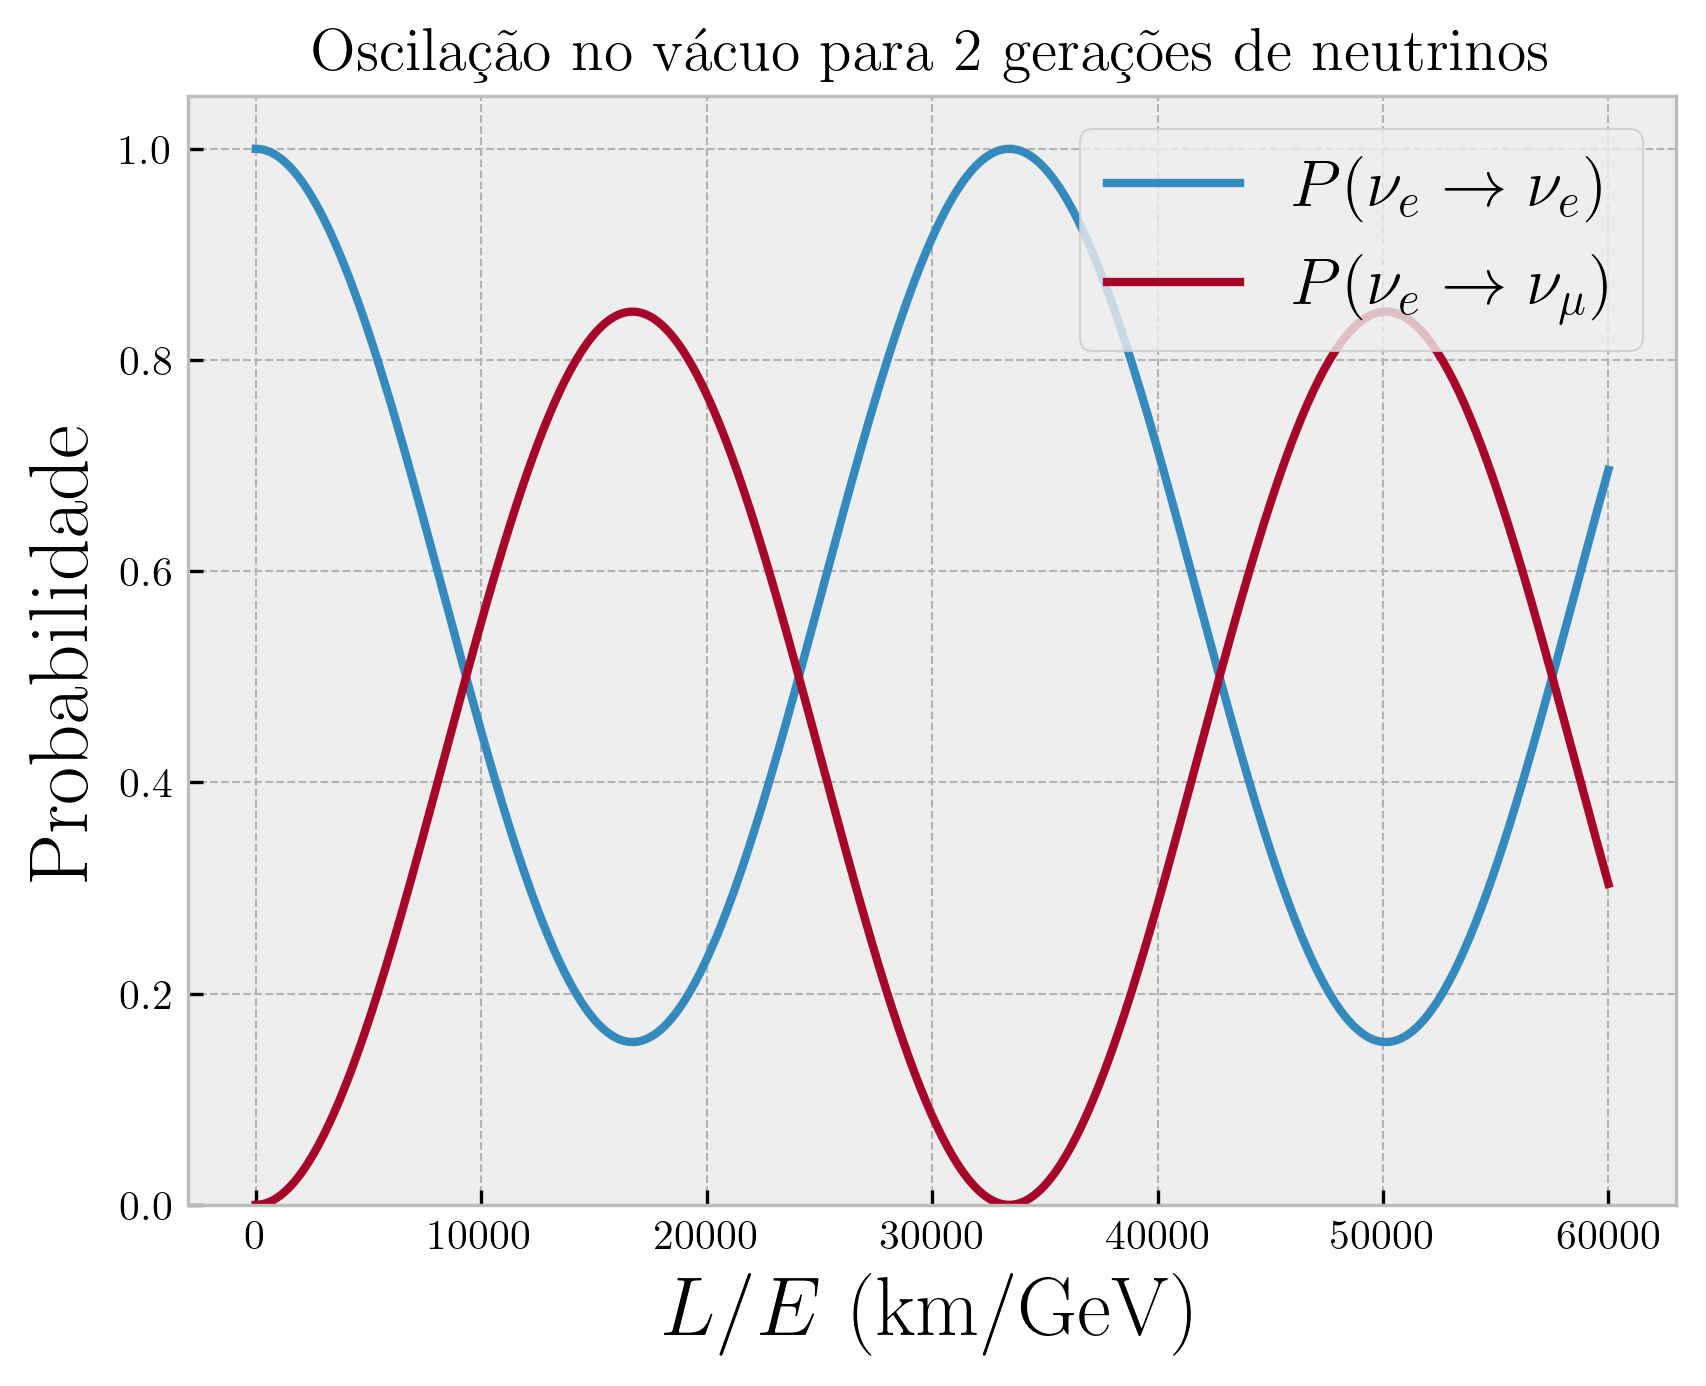
\includegraphics[width=0.52\textwidth]{fig/2nu-vacuo.png}
\caption{Oscilação de sabor no vácuo, com os parâmetros do NuFIT, para duas gerações de neutrinos $\nu_e$ e $\nu_\mu$.}
\label{fig:2nu-vacuo}
\end{figure}


\section{Oscilação de três neutrinos no vácuo} \label{sec:3nu-vacuo}


A relação \ref{eq:unitaria} vale para qualquer número de neutrinos, já que se trata de uma simples mudança de base. Porém, para três neutrinos, a matriz unitária de mistura $U$ é $3 \times 3$ e já não assume uma forma tão simples quanto a da equação \ref{eq:mix2}. A parametrização mais convencional usada na literatura é dada pela matriz de mistura de Maki-Nakagawa-Sakata (Seção VII de \cite{gonzalez})
\begin{equation} \label{eq:mixmatrix}
U =
\begin{pmatrix}
c_{12} c_{13} & s_{12} c_{13} & s_{13} e^{-i\dcp} \\
-s_{12}c_{23} - c_{12}s_{23}s_{13}e^{i\dcp} & c_{12}c_{23} - s_{12}s_{23}s_{13} \, e^{i\dcp} & s_{23}c_{13} \\
s_{12}s_{23} - c_{12}c_{23}s_{13}e^{i\dcp} & -c_{12}s_{23} - s_{12}c_{23}s_{13} \, e^{i\dcp} & c_{23}c_{13} \\
\end{pmatrix}
\end{equation}
\begin{equation} \label{eq:3matrices}
=
\begin{pmatrix}
1 & 0 & 0 \\
0 & c_{23} & s_{23} \\
0 & -s_{23} & c_{23} \\
\end{pmatrix}
\begin{pmatrix}
c_{13} & 0 & s_{13} \, e^{-i\dcp} \\
0 & 1 & 0 \\
-s_{13} \, e^{i\dcp} & 0 & c_{13} \\
\end{pmatrix}
\begin{pmatrix}
c_{12} & s_{12} & 0 \\
-s_{12} & c_{12} & 0 \\
0 & 0 & 1 \\
\end{pmatrix},
\end{equation}
onde $c_{ij} = \cos(\theta_{ij})$ e $s_{ij} = \sin(\theta_{ij})$, sendo $\theta_{ij}$ o ângulo de mistura entre os neutrinos $\nu_i$ e $\nu_j$, e $\dcp$ é uma fase relacionada à violação da simetria CP de conjugação de carga e paridade.

É possível ver pela equação \ref{eq:3matrices} que a matriz $U$ se trata de uma combinação de três matrizes mais simples, que na verdade são matrizes de misturas de duas gerações de neutrinos (ignorando o termo de fase $\dcp$). Note que a matriz mais à direita da equação \ref{eq:3matrices} é essencialmente a matriz $U$ para dois neutrinos da equação \ref{eq:mix2}. Essa observação é relevante pois, ao resolver a equação de oscilação de neutrinos numericamente, podemos explorar o caso de 2 gerações de neutrinos a partir dos vínculos $\theta_{13} = \theta_{23} = 0$, já que nessa situação a matriz $U$ de 3 gerações se reduz à matriz de 2 gerações.

Novamente, pela equação \ref{eq:mass-eigen}, a matriz $M$ da hamiltoniana na base de autoestados de massa é $M = \frac{1}{2E} \, \text{diag}(m_1^2, m_2^2, m_3^2)$. Agora, assumindo o ordenamento de massas normal $m_1 \leq m_2 \leq m_3$ para simplificar a exposição\footnote{Atualmente, temos conhecimento apenas das diferenças entre as massas ao quadrado, sendo os últimos dados do NuFIT $\Delta m_{21}^2 = 7.42 \cdot 10^{-5} \unit{eV^2}$ e $\Delta m_{3\ell}^2 = 2.515 \cdot 10^{-3} \unit{eV^2}$. Assim, somente existem duas possibilidades para o ordenamento de massas, a ordem normal $m_1 \leq m_2 \leq m_3$ (NO) ou a ordem invertida $m_3 \leq m_1 \leq m_2$ (IO).}, podemos então subtrair a matriz múltipla da identidade $m_2^2 \, I$, $I = \text{diag}(1,1,1)$, já que esta só contribui para uma fase global na evolução do sistema. Assim, vemos que $M = \frac{1}{2E} \, \text{diag}(- \Delta m_{21}^2, 0, \Delta m_{32}^2)$, com $\Delta m_{ij}^2 = m_i^2 - m_j^2$.

De novo, a partir da mudança de base $\H = U M U^\dagger$ podemos obter a hamiltoniana do sistema na base de sabores. Entretanto, devido à forma complicada de $U$ na equação \ref{eq:mixmatrix}, resolver a equação de Schrödinger para $\H$ não ajuda a clarificar o problema, de modo que optamos por resolver a equação diferencial ordinária (EDO) numericamente. Escrevendo $\ket{\nu(t)} = \psi_e(t) \ket{\nu_e} + \psi_\mu(t) \ket{\nu_\mu} + \psi_\tau(t) \ket{\nu_\tau}$, a equação de Schrödinger nos dá
\begin{equation} \label{eq:3nu-vacuo}
i \dv{t}
\begin{pmatrix}
\psi_e \\ \psi_\mu \\ \psi_\tau
\end{pmatrix}
=
\qty[ \frac{1}{2E} \, U
\begin{pmatrix}
-\Delta m_{21}^2 & 0 & 0 \\
0 & 0 & 0 \\
0 & 0 & \Delta m_{32}^2 \\
\end{pmatrix}
\, U^\dagger ]
\begin{pmatrix}
\psi_e \\ \psi_\mu \\ \psi_\tau
\end{pmatrix}.
\end{equation}

Descreveremos no Apêndice \ref{sec:numeric} os passos para transformar a equação \ref{eq:3nu-vacuo} de valores complexos para uma equação real e então utilizaremos o Python para resolvê-la.

Manipulando as condições iniciais $\ket{\nu(t)} = \ket{\nu_\alpha}$, $\alpha = e, \mu, \tau$, e utilizando os parâmetros do NuFIT de Outubro de 2021, temos os seguintes gráficos para três gerações de neutrinos com as probabilidades de transições $P(\nu_\alpha \to \nu_e), P(\nu_\alpha \to \nu_\mu)$ e $P(\nu_\alpha \to \nu_\tau)$. Os pares de gráficos representam a mesma curva, com a diferença de que os da direita apenas mostram a oscilação durante uma curta distância percorrida (os da direita são apenas os inícios dos gráficos da esquerda).

\begin{figure}[H]
\centering
\begin{subfigure}{.5\textwidth}
  \centering
  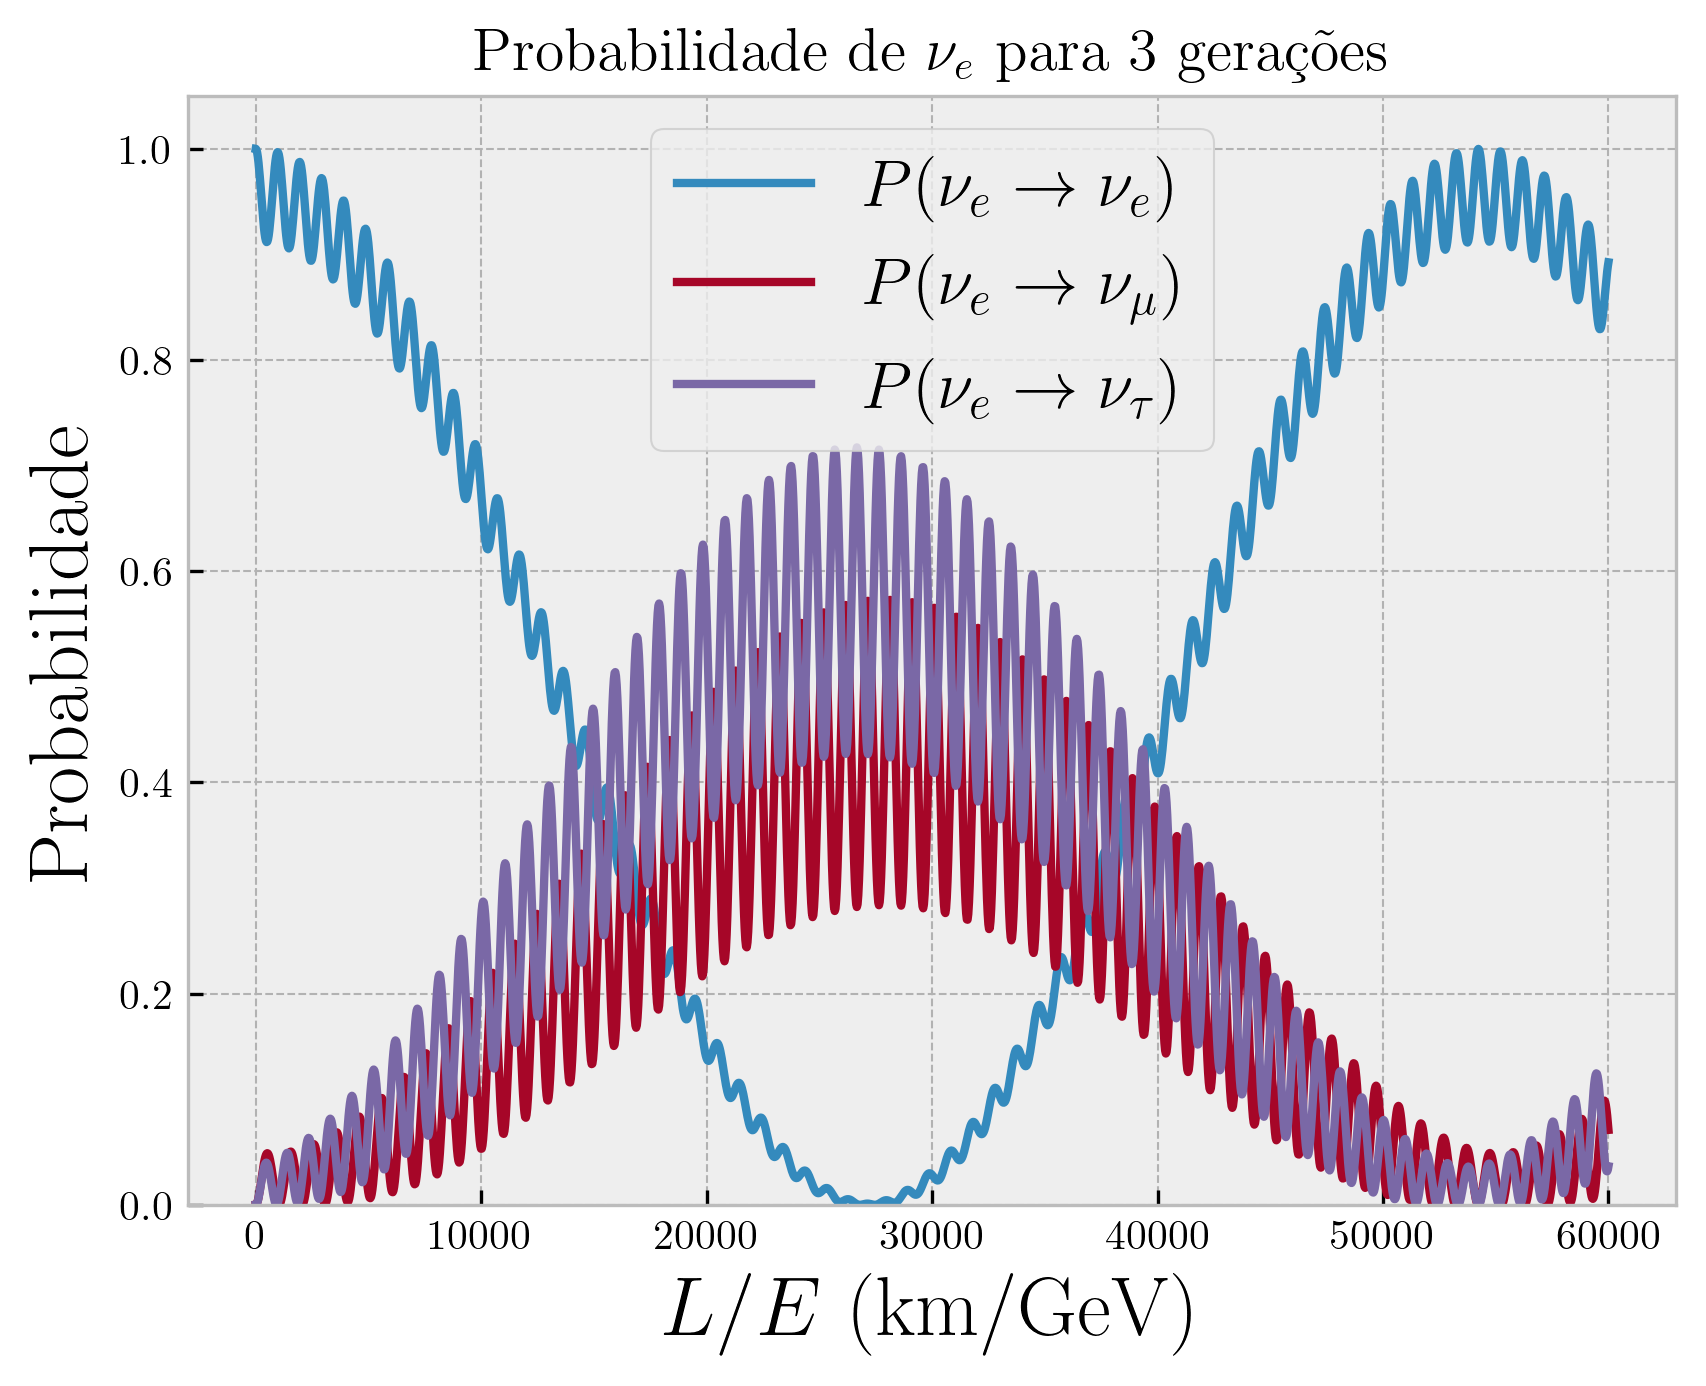
\includegraphics[width=.75\linewidth]{fig/3nu-vacuo-e.png}
  \caption{}
  \label{fig:vacuo-e}
\end{subfigure}%
\begin{subfigure}{.5\textwidth}
  \centering
  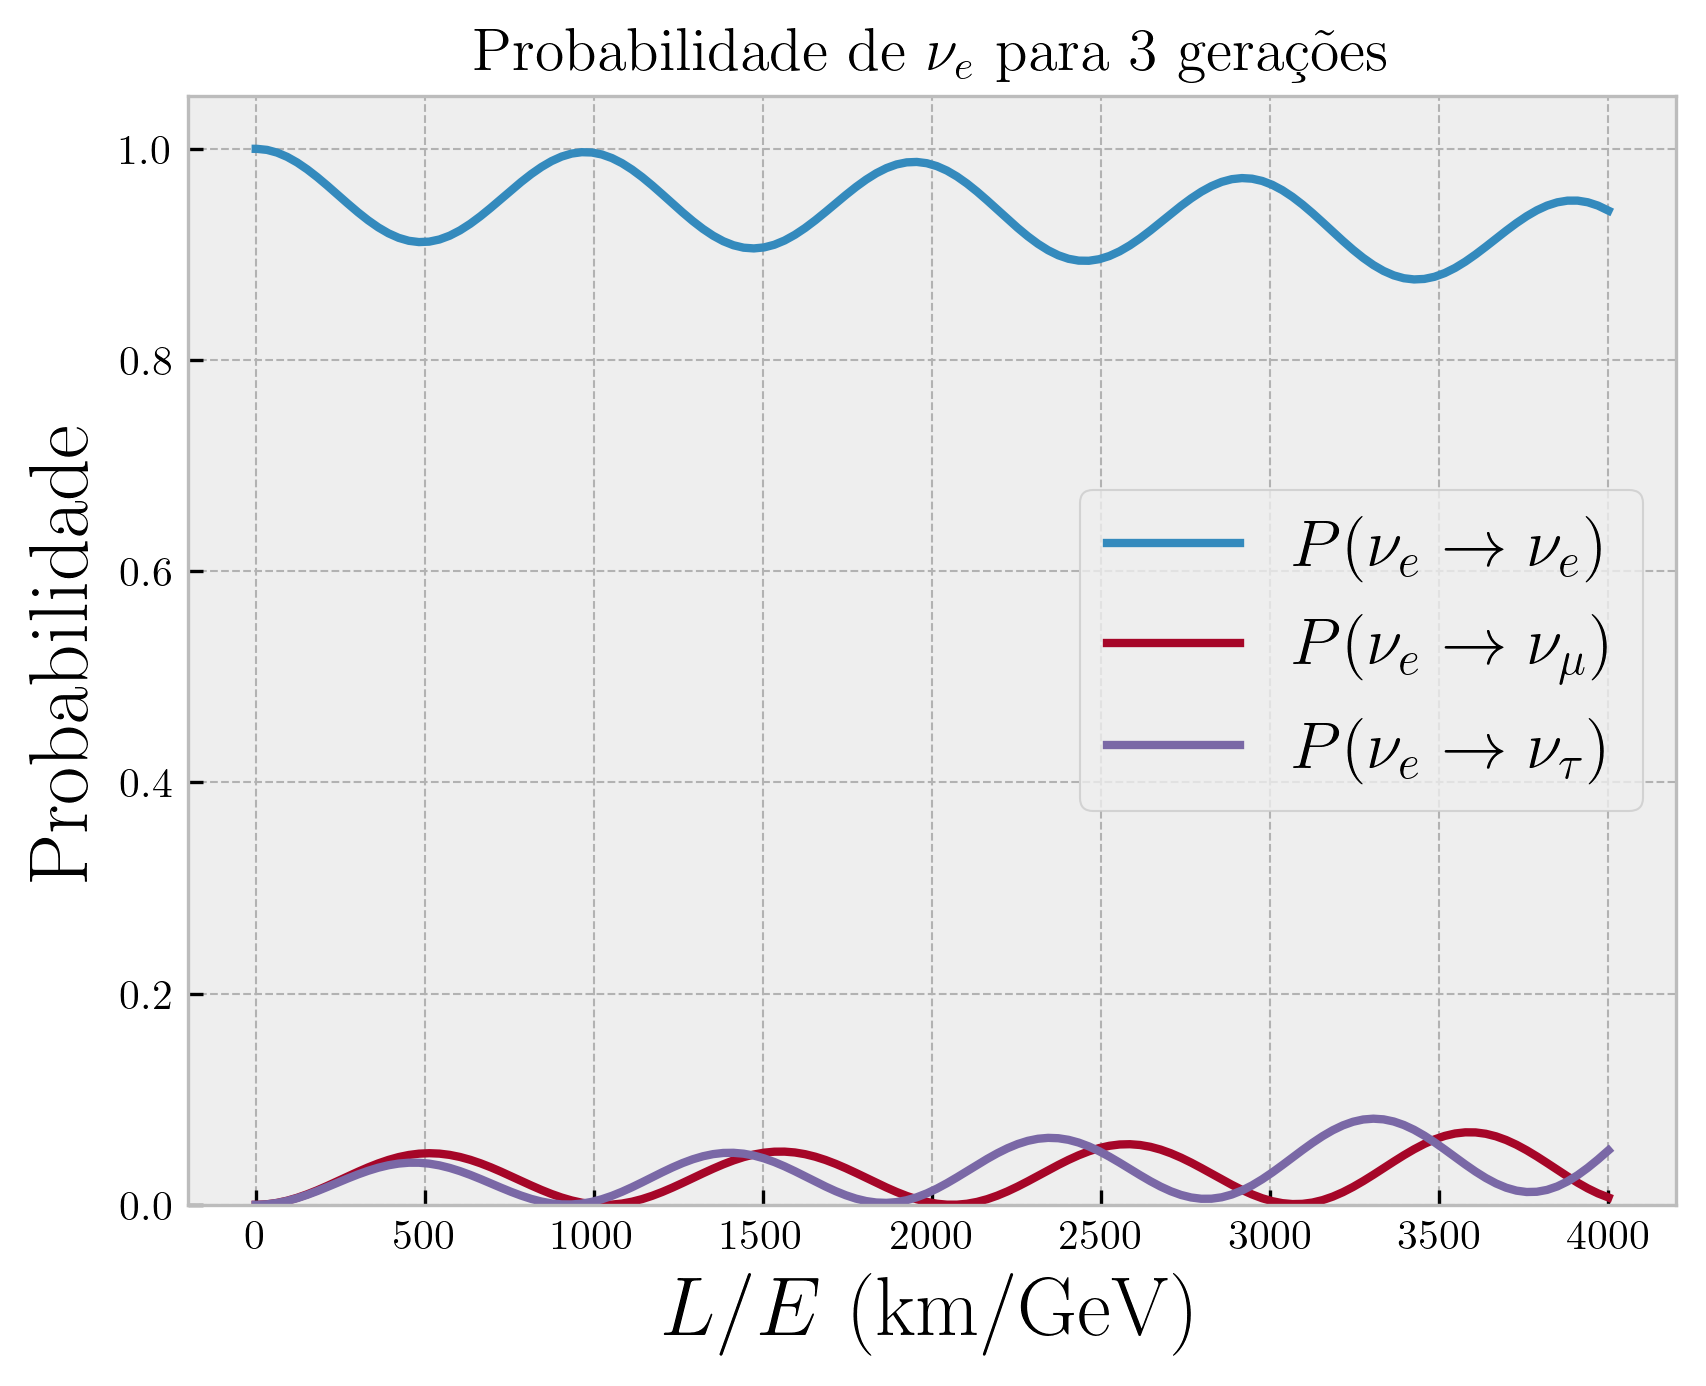
\includegraphics[width=.75\linewidth]{fig/3nu-vacuo-e_short.png}
  \caption{}
  \label{fig:vacuo-e_short}
\end{subfigure}
\caption{Probabilidades de transição de um neutrino $\nu_e$ no vácuo.}
\label{fig:vacuo_electron}
\end{figure}

\begin{figure}[H]
\centering
\begin{subfigure}{.5\textwidth}
  \centering
  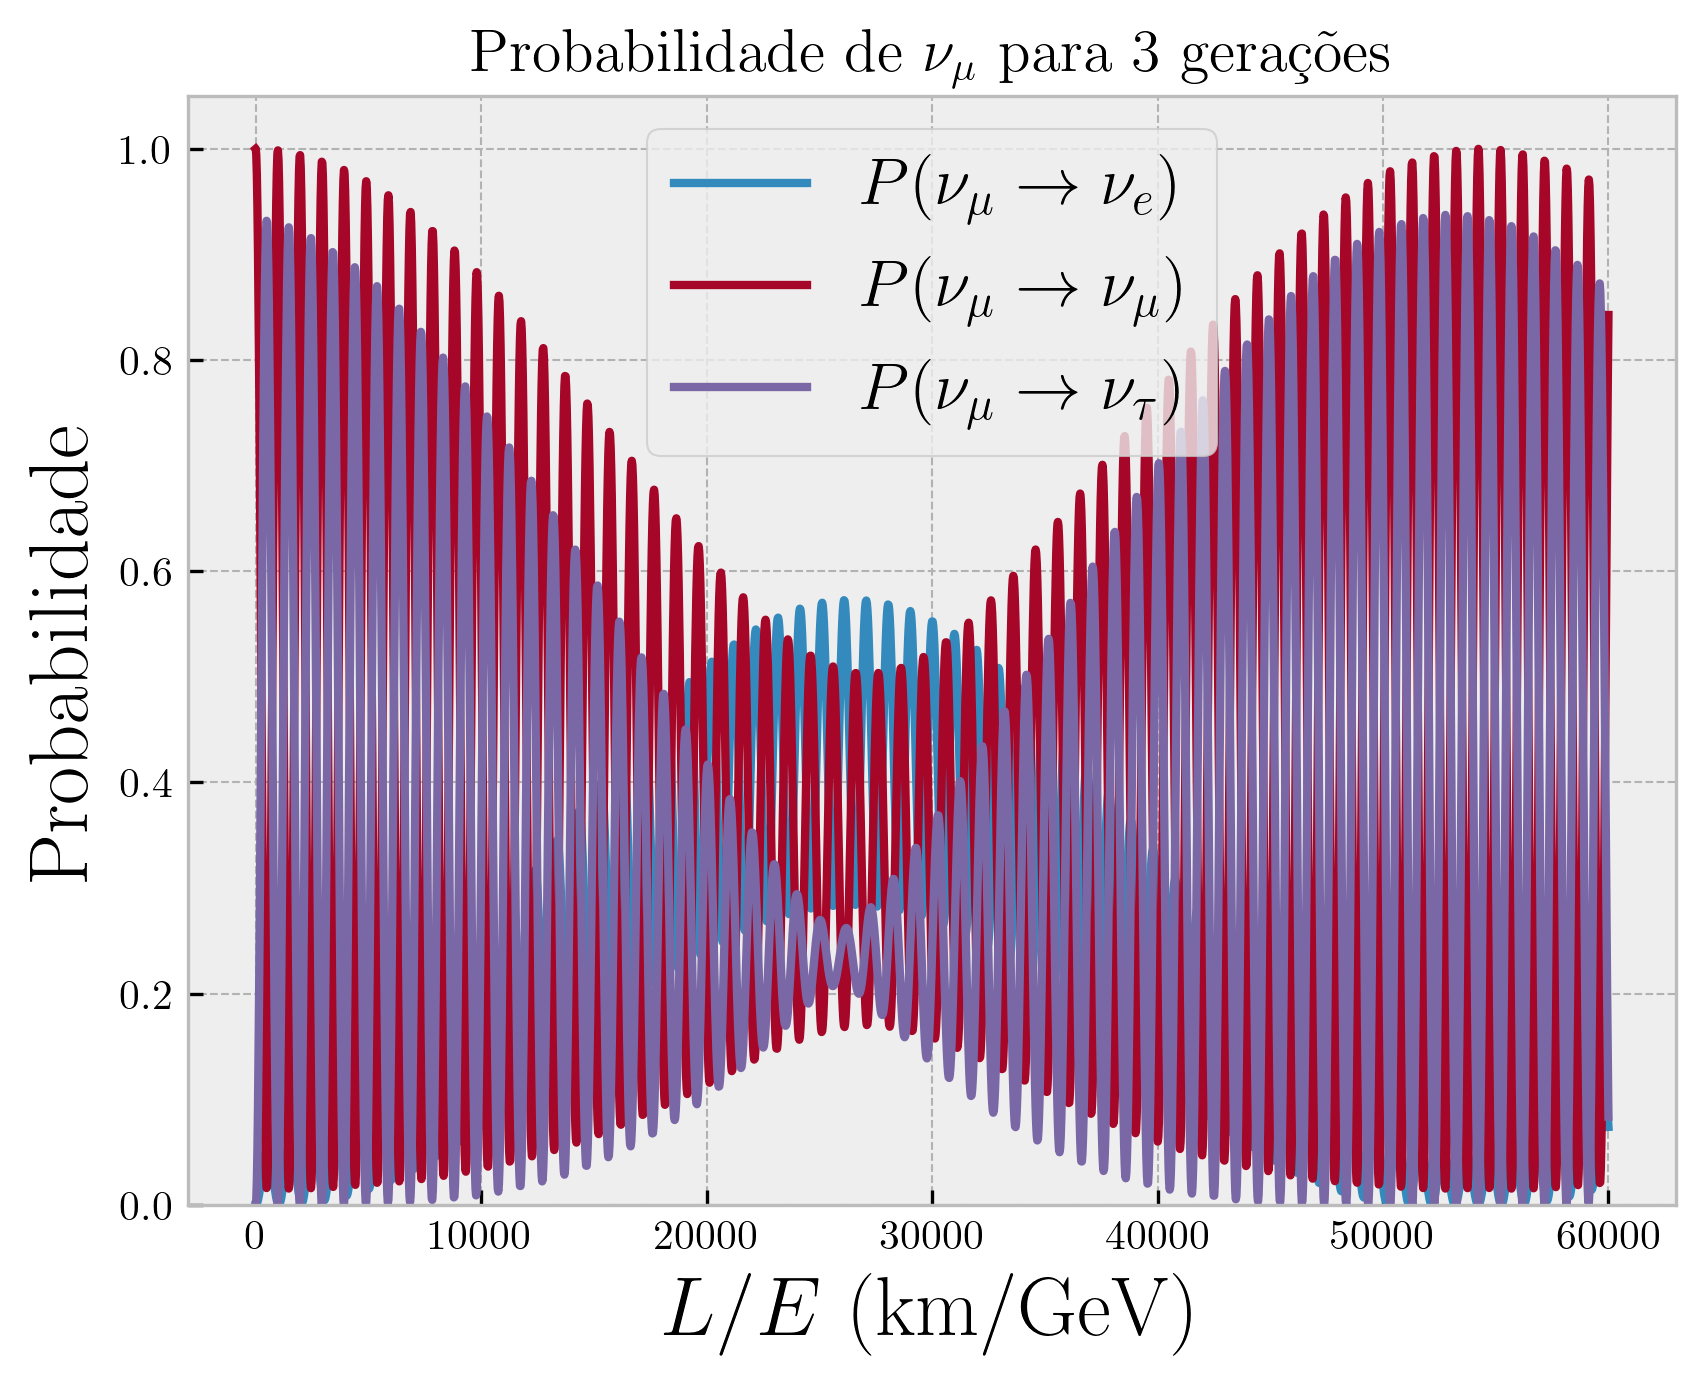
\includegraphics[width=.75\linewidth]{fig/3nu-vacuo-mu.png}
  \caption{}
  \label{fig:vacuo-mu}
\end{subfigure}%
\begin{subfigure}{.5\textwidth}
  \centering
  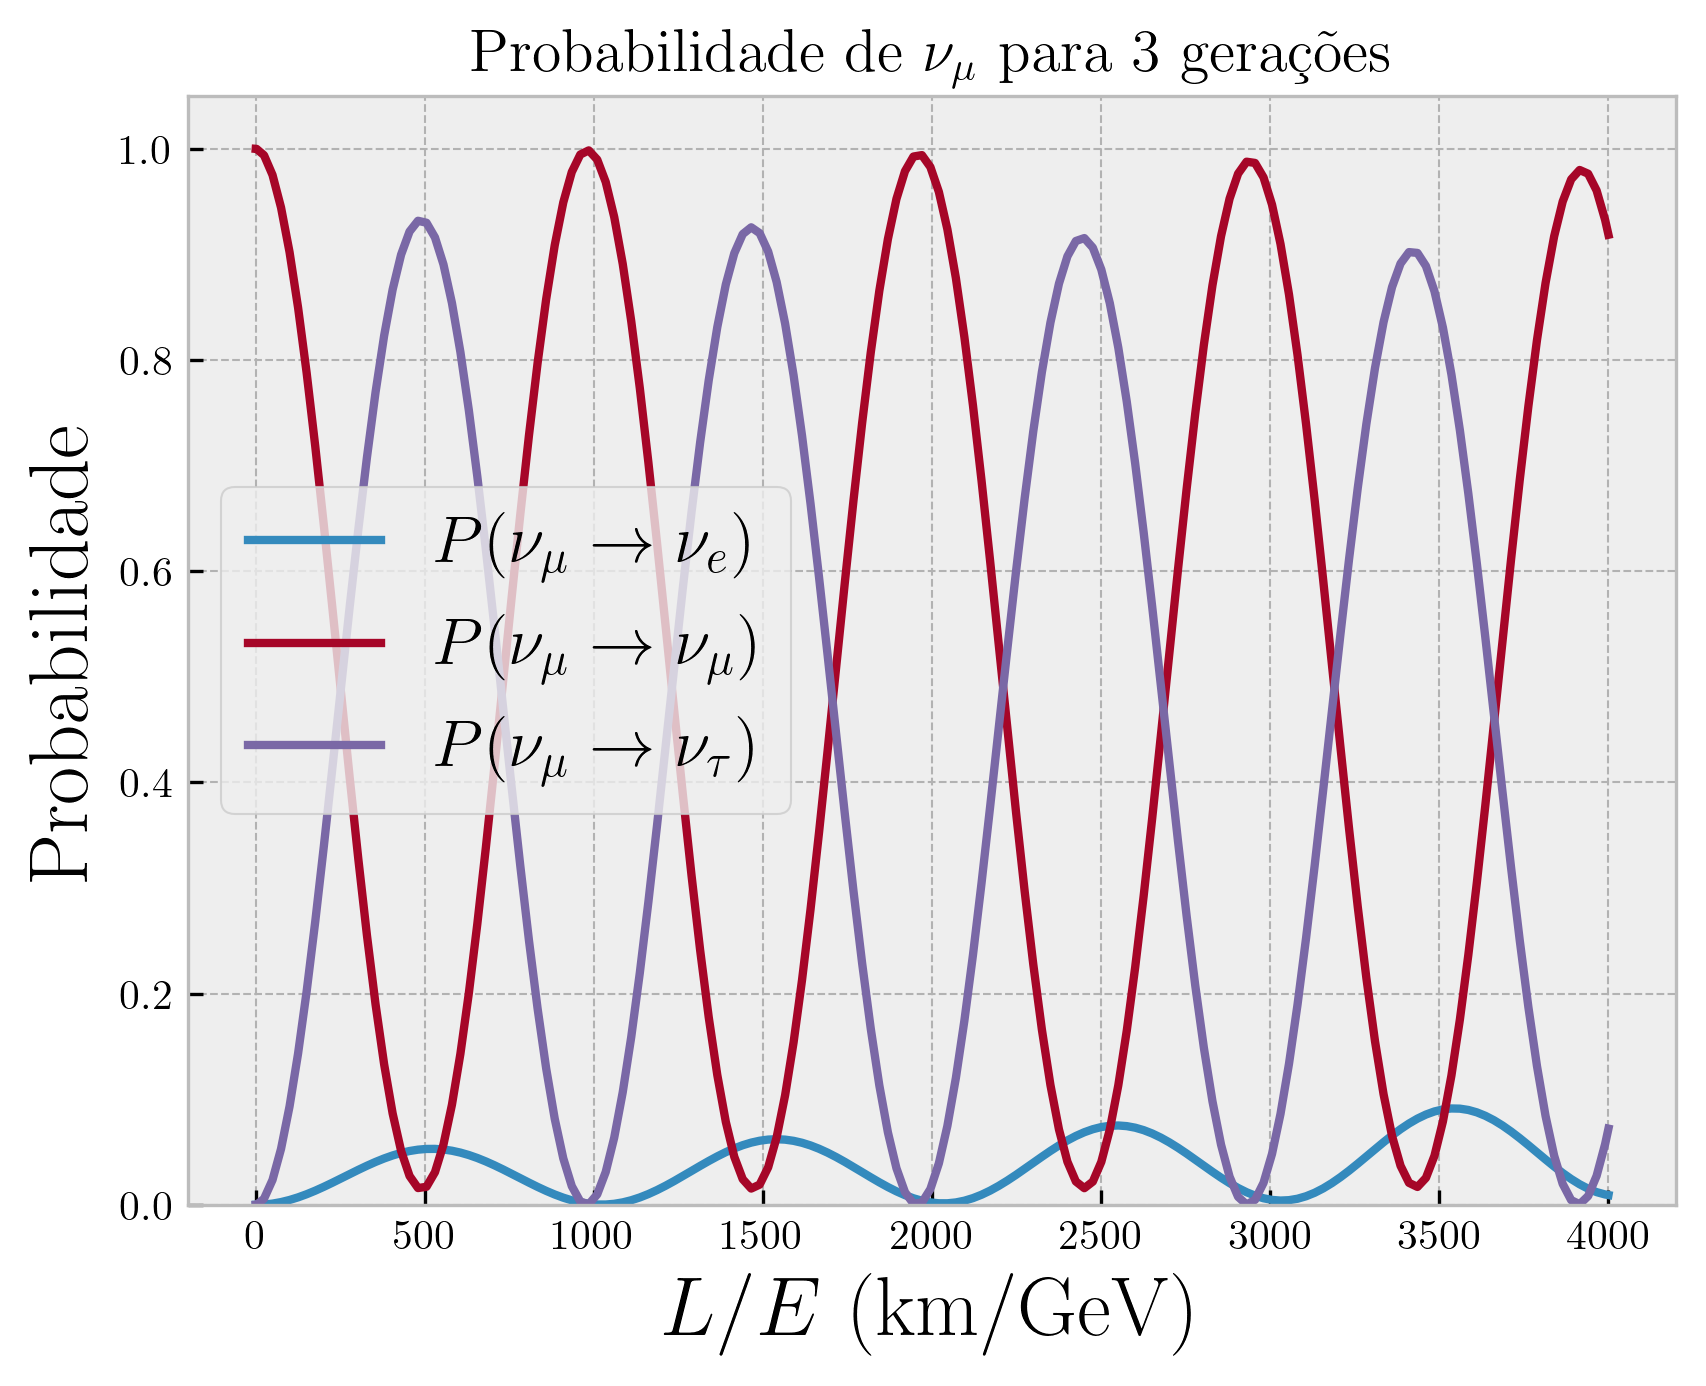
\includegraphics[width=.75\linewidth]{fig/3nu-vacuo-mu_short.png}
  \caption{}
  \label{fig:vacuo-mu_short}
\end{subfigure}
\caption{Probabilidades de transição de um neutrino $\nu_\mu$ no vácuo.}
\label{fig:vacuo_muon}
\end{figure}

\begin{figure}[H]
\centering
\begin{subfigure}{.5\textwidth}
  \centering
  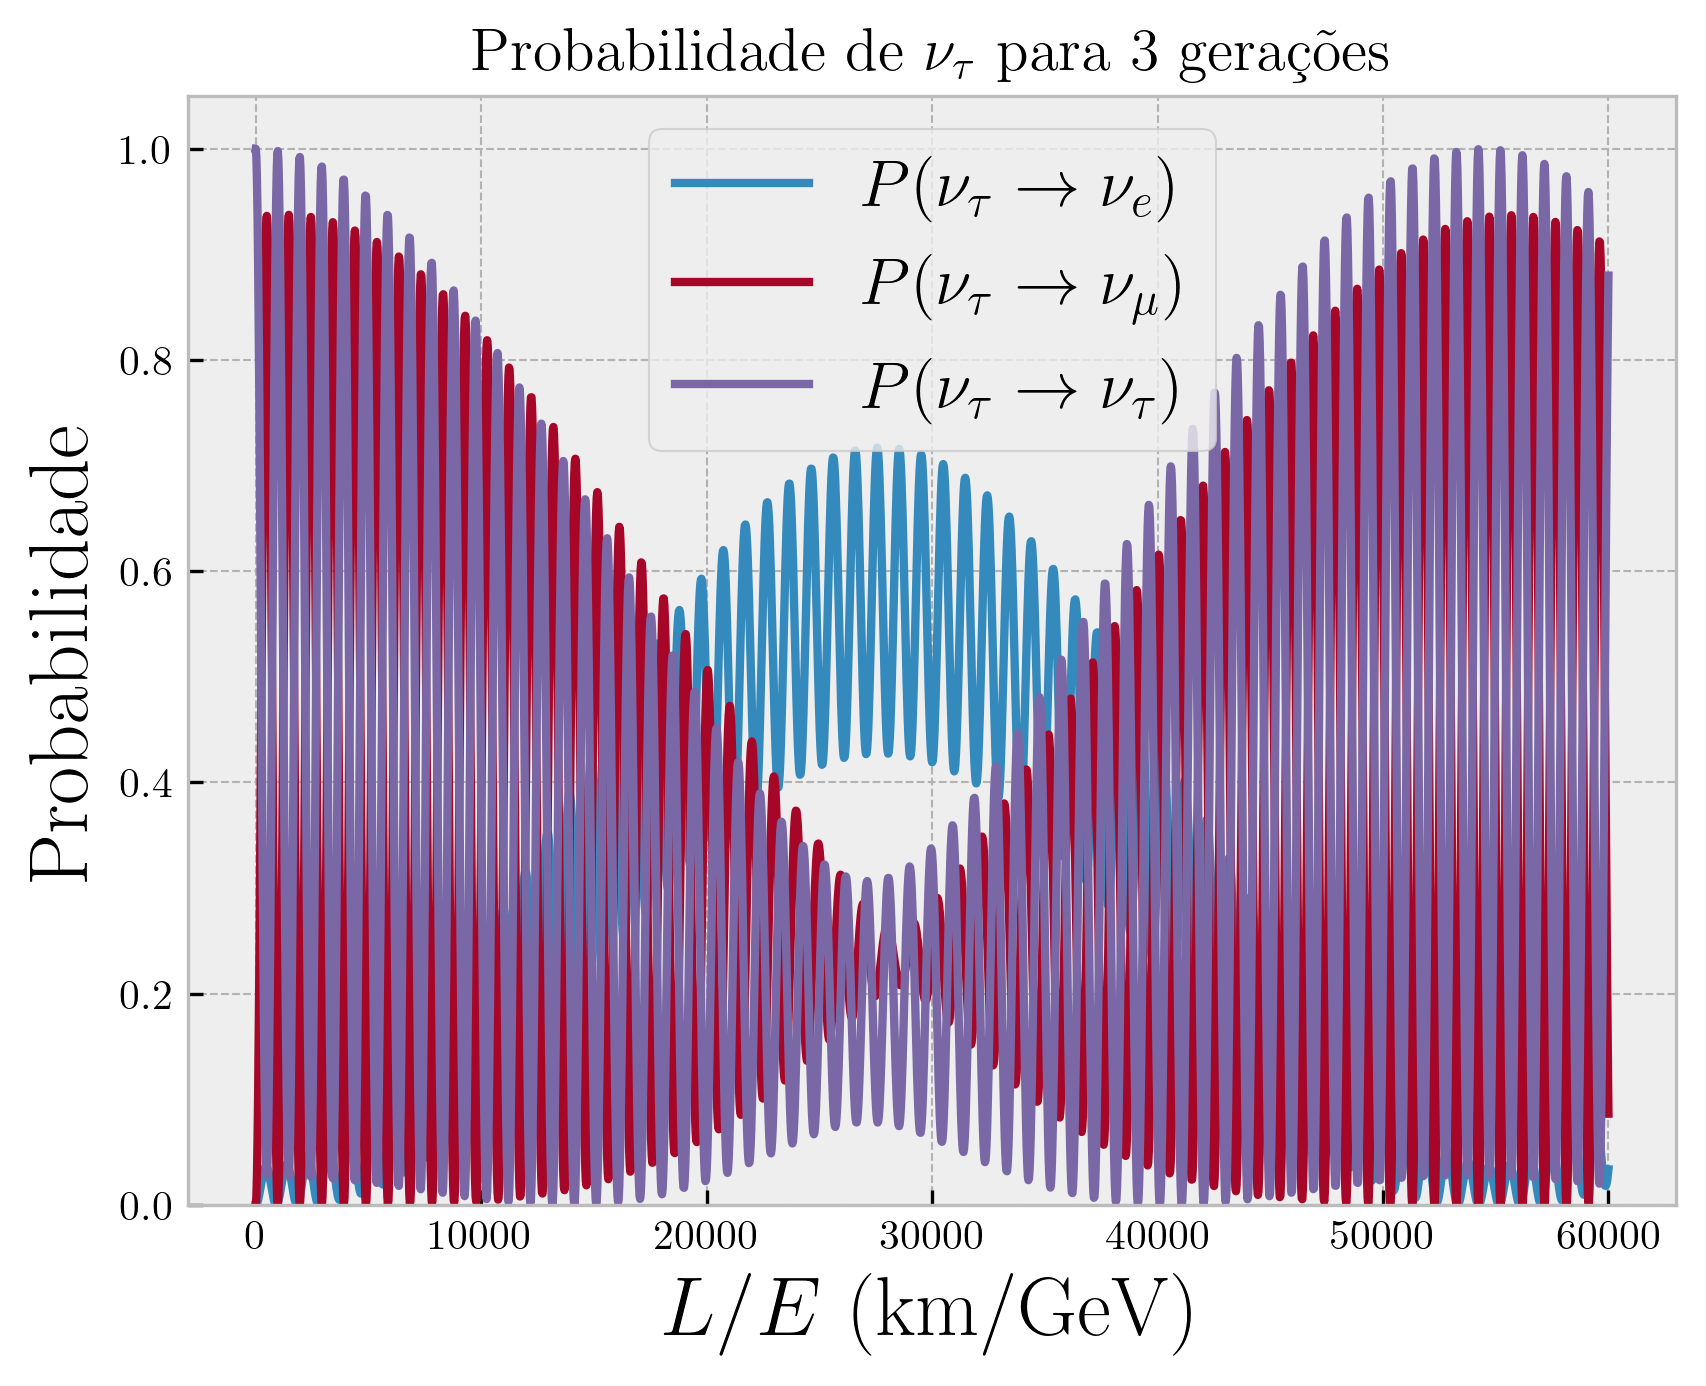
\includegraphics[width=.75\linewidth]{fig/3nu-vacuo-tau.png}
  \caption{}
  \label{fig:vacuo-tau}
\end{subfigure}%
\begin{subfigure}{.5\textwidth}
  \centering
  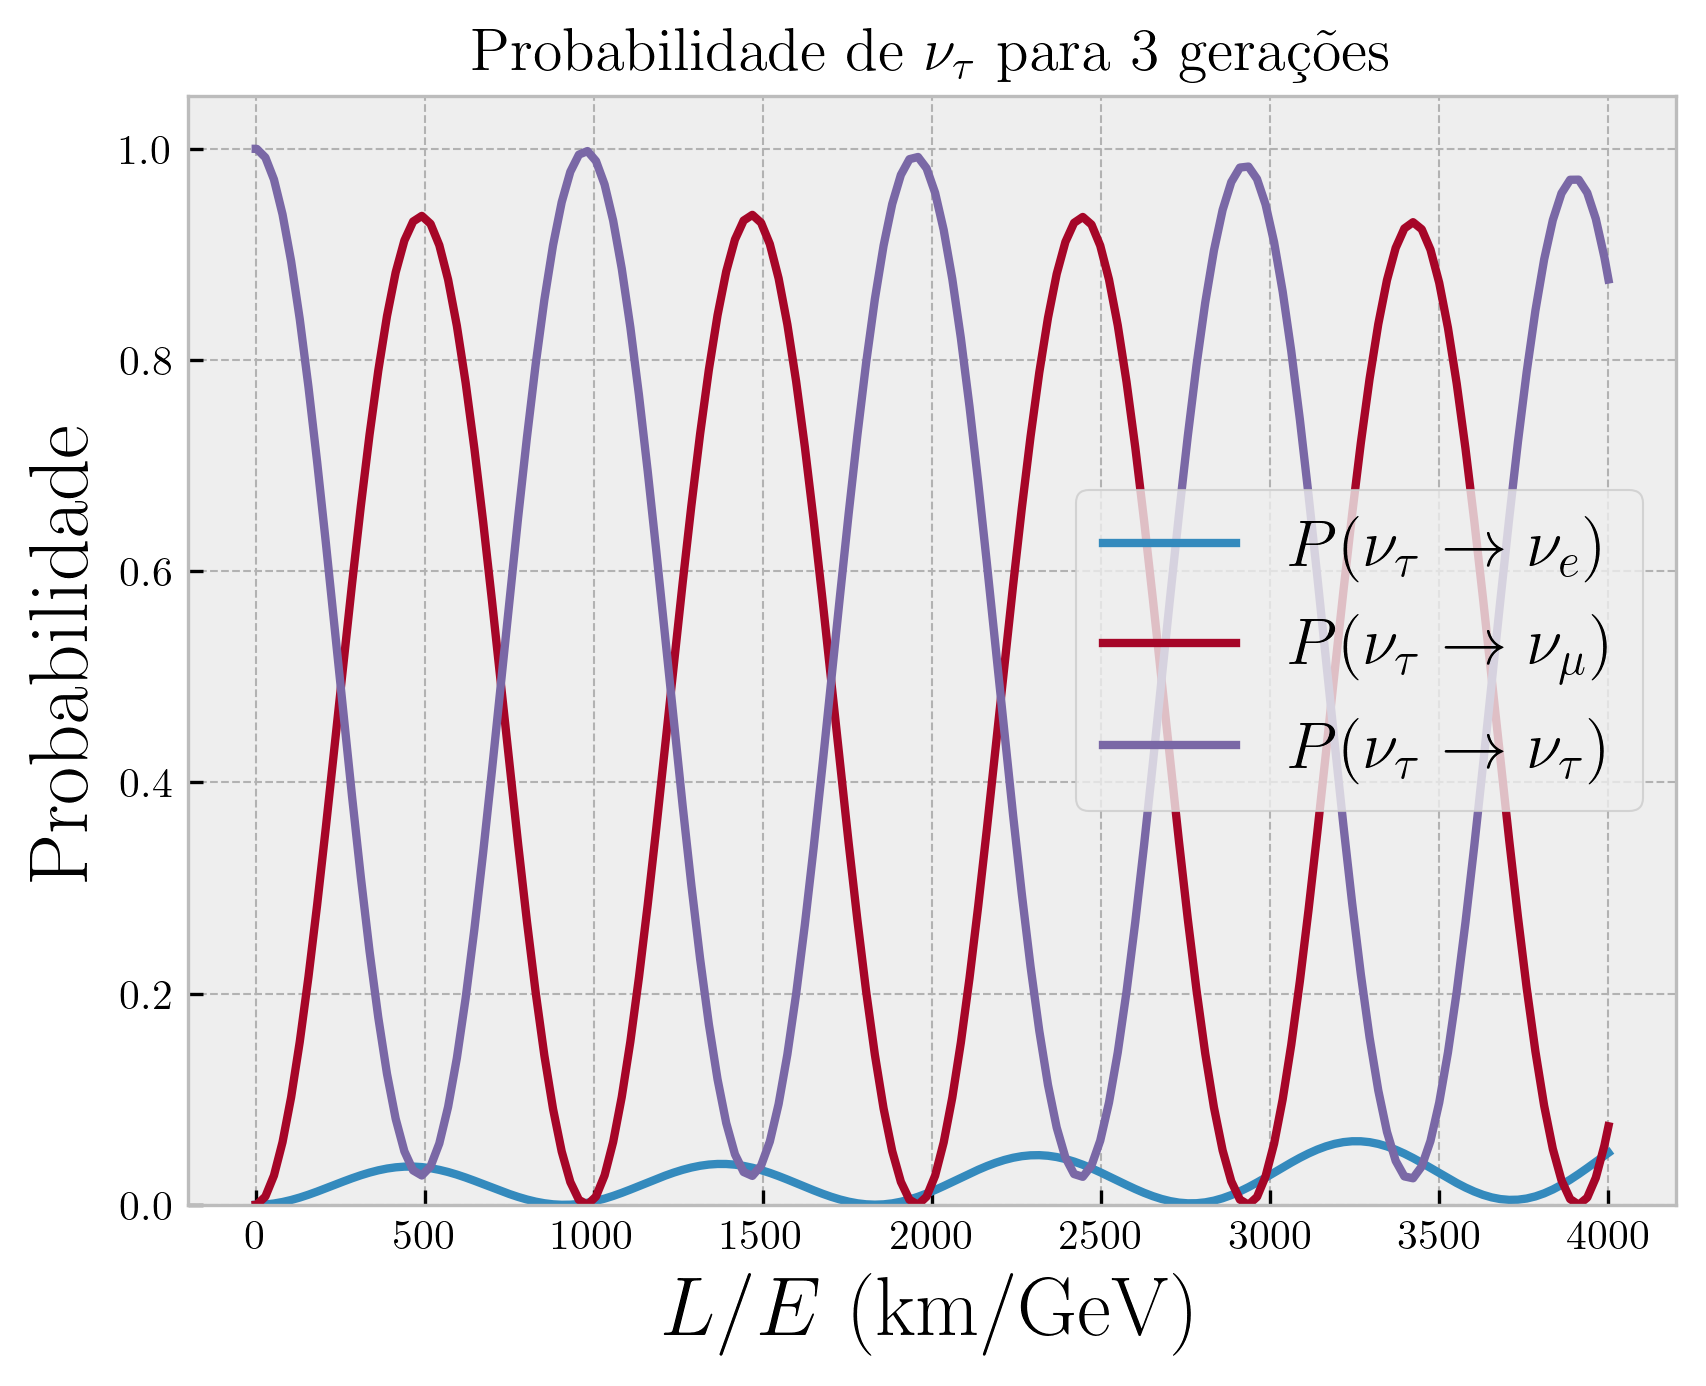
\includegraphics[width=.75\linewidth]{fig/3nu-vacuo-tau_short.png}
  \caption{}
  \label{fig:vacuo-tau_short}
\end{subfigure}
\caption{Probabilidades de transição de um neutrino $\nu_\tau$ no vácuo.}
\label{fig:vacuo_tau}
\end{figure}

É evidente que a consideração do neutrino $\nu_\tau$ adicional modifica significativamente as oscilações observadas na Figura \ref{fig:2nu-vacuo}, que retrata o caso de 2 gerações. Observamos uma oscilação de frequência maior e outra de frequência menor em todos as Figuras \ref{fig:vacuo_electron}, \ref{fig:vacuo_muon} e \ref{fig:vacuo_tau}, sendo que os gráficos \ref{fig:vacuo-mu} e \ref{fig:vacuo-tau} de longo alcance relativas às condições iniciais de $\nu_\mu$ e $\nu_\tau$ apresentam claramente o fenômeno de batimento, onde vemos grupos de onda bem definidos. Outra coisa a se notar é que as Figuras \ref{fig:vacuo-mu_short} e \ref{fig:vacuo-tau_short} são bastante similares, o que nos indica que, durante um intervalo de tempo curto, as oscilações de $\nu_\mu$ e $\nu_\tau$ são bem próximas. Isso pode ser explicado pelo fato das diferenças de massas ao quadrado $7.42 \times 10^{-5} \unit{eV^2} = \Delta m_{21}^2 \ll \Delta m_{32}^2 = 2.515 \times 10^{-3} \unit{eV^2}$ serem separadas por duas ordens de grandeza, ou seja, temos que $\Delta m_{31}^2 = \Delta m_{32}^2 + \Delta m_{21}^2 \approx \Delta m_{32}^2$. Pelo fato de $\Delta m_{31}^2$ e $\Delta m_{32}^2$ serem muito próximos, em pequenas distâncias percorridas pelo neutrino, existe uma simetria entre $\nu_\mu$ e $\nu_\tau$, que explica a similaridade entre as Figuras \ref{fig:vacuo-mu_short} e \ref{fig:vacuo-tau_short}.

\section{Neutrinos solares} \label{sec:nu-solar}

Antes de discutirmos a interação entre os neutrinos na matéria, consideremos o espalhamento mais simples $e^- e^- \to e^- e^-$. Baseando-nos na Seção 4.8 de \cite{peskin}, temos que o diagrama de Feynman de maior contribuição para esse processo é

\begin{figure}[H]
\centering
\feynmandiagram [horizontal=a to b] {
  i1 [particle=\(e^-\)] -- [fermion, edge label'=\(p\)] a -- [fermion, edge label'=\(p'\)] i2 [particle=\(e^-\)],
  a -- [photon, edge label=\(\gamma\)] b,
  f1 [particle=\(e^-\)] -- [anti fermion, edge label'=\(k'\)] b -- [anti fermion, edge label'=\(k\)] f2 [particle=\(e^-\)],
};
\caption{Diagrama de Feynman de menor ordem para $e^- e^- \to e^- e^-$.}
\label{fig:electron-electron}
\end{figure}
Sendo $\gamma^\mu$ as matrizes de Dirac, $u$ a solução de onda plana para a equação de Dirac do elétron e $-i g_{\mu\nu}/q^2$ o propagador de Feynman, a amplitude invariante é dada por
$$
-i\s{M} = \Big[ie \, \cc{u}(p') \gamma^\mu u(p)\Big] \,
\qty[\frac{- i g_{\mu \nu}}{q^2}] \,
\Big[ie \, \cc{u}(k') \gamma^\nu u(k)\Big] ,
\quad q = p - p' = k' - k,
$$
\begin{equation} \label{eq:ampli-ee}
\s{M} =
\Big[\cc{u}(p') \gamma^\mu u(p)\Big] \, \,
\qty(\frac{- e^2}{q^2}) \,
\Big[\cc{u}(k') \gamma_\mu u(k)\Big] ,
\end{equation}
onde $j^\mu = \cc{\psi} \gamma^\mu \psi$ é a corrente fermiônica e possui forma\footnote{Dizemos que $A^\mu$ tem forma $V$ (de vetor) se sua expressão tiver um termo $\gamma^\mu$ e que tem forma $A$ (vetor axial) se ele possuir o termo $\gamma^\mu \gamma^5$} de operador vetorial $V$, de maneira que podemos escrever $\s{M} = -e^2/q^2 \, J^\mu J_\mu^\dagger$.

\subsection{Interação fraca} \label{sec:weak-int}

Baseando-se nas discussões da Seção 12 de \cite{halzen} e Seção 22.2 de \cite{schwartz}, em 1933 o físico Enrico Fermi investigou a reação \ref{eq:beta} do decaimento $\beta$, propondo que sua forma cruzada
\begin{equation} \label{eq:beta-crossed}
p^+ + e^- \to n^0 + \nu_e
\end{equation}
fosse modelada em analogia com a forma corrente-corrente da amplitude \ref{eq:ampli-ee}. Sua teoria fenomenológica utilizava a amplitude invariante
\begin{equation} \label{eq:fermi-ampli}
\s{M} = \Big[ \cc{u}_n \gamma^\mu u_p \Big] \Big( G_F \Big) \Big[ \cc{u}_{\nu_e} \gamma^\mu u_e \Big],
\end{equation}
onde $G_F$ é a chamada constante de Fermi e a corrente $j^\mu = \cc{\psi} \gamma^\mu \psi$ novamente tem forma de um operador vetorial $V$.

Esta foi conhecida como a teoria 4-Fermi (Seção 29.4 de \cite{schwartz}) e se mostrou uma descrição efetiva para a interação fraca à baixas energias. Porém, como foi apontado mais tarde em 1956 por Lee e Yang (Seção 12.1 de \cite{halzen}), que se basearam em uma coleção de experimentos de interação fraca, a simetria de paridade não deve ser conservada nesta interação. Essa observação requer uma modificação na equação \ref{eq:fermi-ampli} proposta por Fermi, o que levou à forma $V-A$ (vetor menos vetor axial) da corrente fraca $J^\mu = \cc{\psi} \, \gamma^\mu \frac{1}{2} (1 - \gamma^5) \, \psi$ e na amplitude
\begin{equation} \label{eq:weak-ampli}
\s{M} = \frac{4 \, G_F}{\sqrt{2}} \,
\qty[ \cc{u}_n \gamma^\mu \, \frac{1}{2} (1 - \gamma^5) u_p ]
\qty[ \cc{u}_{\nu_e} \gamma_\mu \, \frac{1}{2} (1 - \gamma^5) u_e ] .
\end{equation}

A equação \ref{eq:weak-ampli} ainda se trata de uma teoria efetiva para a interação fraca. Como será estudado com mais detalhes no resto deste projeto, a força fraca acontece por meio dos bósons vetoriais $W^{\pm}$ e $Z^0$, sendo o propagador dado por\footnote{Seção 6.12 de \cite{halzen}}
\begin{equation} \label{eq:boson-propagator}
\frac{i (- g^{\mu \nu} + p^{\mu} p^{\nu} / M^2)}{p^2 - M^2}.
\end{equation}

Apesar disso, a amplitude \ref{eq:weak-ampli} se trata de uma excelente aproximação para a interação fraca a baixas energias, uma condição que é obedecida na interação de neutrinos da reação $^8$B no interior do Sol. De fato, temos que suas energias chegam somente até a ordem de $15 \unit{MeV}$ (como pode ser visto na Figura \ref{fig:nu8b-energy}). Enquanto isso, considerando como predominantes as interações de corrente carregada (troca do bóson $W$), temos que a massa do bóson $W$ é da ordem de $M = 80 \unit{GeV}$. Fazendo a aproximação $p^2 \ll M^2$, o propagador \ref{eq:boson-propagator} se reduz a uma constante, o que recupera o perfil da amplitude \ref{eq:weak-ampli}.


\subsection{Potencial de interação} \label{sec:potencial-int}

Seguindo a seção III.B de \cite{gonzalez}, utilizando como referência a amplitude da equação \ref{eq:weak-ampli} e nos restringindo a interações de corrente carregada, podemos usar a seguinte hamiltoniana efetiva a baixas energias $H_W$ para descrever o potencial efetivo da evolução de um neutrino $\nu_e$ na interação com um elétron:
$$
H_W = \frac{G_F}{\sqrt{2}}
\Big[ \cc{\nu_e}(x) \gamma^\mu (1 - \gamma^5) e(x)\Big]
\Big[ \cc{e}(x) \gamma_\mu (1 - \gamma^5) \nu_e(x)\Big],
$$
onde $e(x)$ e $\nu_e(x)$ são os campos do elétron e do neutrino, respectivamente.

Para obter a hamiltoniana devido a todos os elétrons no meio, temos que tomar a média
$$
H_C^{(e)} = \frac{G_F}{\sqrt{2}} \int \dd[3]{p_e} f(E_e, T)
\Big\langle \ev**{\cc{e}(x) \gamma^\mu (1-\gamma^5) \nu_e(x)
\cc{\nu_e}(x) \gamma_\mu (1-\gamma^5) e(x)}{e(s, p_e)} \Big\rangle,
$$
onde $\Big\langle \cdots \Big\rangle$ denota a média sobre todos os spins $s$ e elétrons de momento $p_e$ no meio e $f(E_e, T)$ é função distribuição de energia dos elétrons no meio.

Assumindo que $f(E_e, T)$ seja homogênea, isotrópica, normalizada; que o meio tenha o mesmo número de elétrons de spin $+1/2$ e $-1/2$; e reconhecendo que as colisões de relevância para o efeito da matéria sobre os neutrinos são apenas as elásticas e coerentes, de acordo com \cite{gonzalez} é possível obter que
$$
H_C^{(e)} = \frac{G_F N_e}{\sqrt{2}} \, \cc{\nu_e}(x) \gamma_0 (1-\gamma_5) \nu_e(x),
$$
onde $N_e$ é a densidade eletrônica e o potencial efetivo $V_e$ para $\nu_e$ pode ser calculado através de uma perturbação de primeira ordem
\begin{equation} \label{eq:potencial}
V_e = \int \dd[3]{x} \ev{H_C^{(e)}}{\nu_e} = \sqrt{2} G_F N_e.
\end{equation}

Para neutrinos solares, a equação \ref{eq:potencial} nos dá a descrição do efeito da matéria sobre a oscilação de sabor.


\subsection{Oscilação na matéria} \label{sec:matter-osc}

Para uma geração de 3 neutrinos oscilando na matéria, a evolução é bem parecida com a equação \ref{eq:3nu-vacuo}. A única diferença é na hamiltoniana, que terá o termo $V_e$ extra somente em sua componente $\ket{\nu_e}$, já que o neutrino $\nu_e$ do elétron é o único que interagirá com a densidade eletrônica no Sol.

Com a adição do termo diagonal $\text{diag}(\sqrt{2} G_F N_e(L), 0,0)$ nossa equação tem uma hamiltoniana dependente de $t = L$:
\begin{equation} \label{eq:evol}
i \dv{t}
\begin{pmatrix}
\psi_e \\ \psi_\mu \\ \psi_\tau
\end{pmatrix}
= \qty[ \frac{1}{2E} \; U
\begin{pmatrix}
-\Delta m_{21}^2 & 0 & 0 \\
0 & 0 & 0 \\
0 & 0 & \Delta m_{31}^2 \\
\end{pmatrix}
U^\dagger +
\begin{pmatrix}
\sqrt{2} \, G_F N_e(t) & 0 & 0 \\
0 & 0 & 0 \\
0 & 0 & 0 \\
\end{pmatrix}
]
\begin{pmatrix}
\psi_e \\ \psi_\mu \\ \psi_\tau
\end{pmatrix},
\end{equation}
onde $U$ é dada pela equação \ref{eq:mixmatrix}.


\subsection{Dados e análises} \label{sec:analise}

Faremos a análise da evolução \ref{eq:evol} com base na interpolação da densidade eletrônica, onde através do \texttt{scipy} obteremos a função $N_e(t)$ interpolada a partir dos dados do modelo solar \href{http://www.sns.ias.edu/~jnb/SNdata/sndata.html#bs2005}{\texttt{BS2005}} \cite{bahcall-model} do website de John N. Bahcall.

Nos restringindo aos neutrinos solares produzidos pela reação do $^8$B, as Figuras \ref{fig:nu8b-energy} e \ref{fig:nu8b-raio} apresentam, respectivamente, os gráficos das densidades de probabilidade $p_E$ e $p_r$ de um neutrino $^8$B ser produzido com energia $E$ e na distância $R = r \, R_{\odot}$ do centro do Sol, sendo $R_\odot = 6.957 \times 10^8 \unit{m}$ o raio solar.

\begin{figure}[H]
\centering
\begin{subfigure}{.5\textwidth}
  \centering
  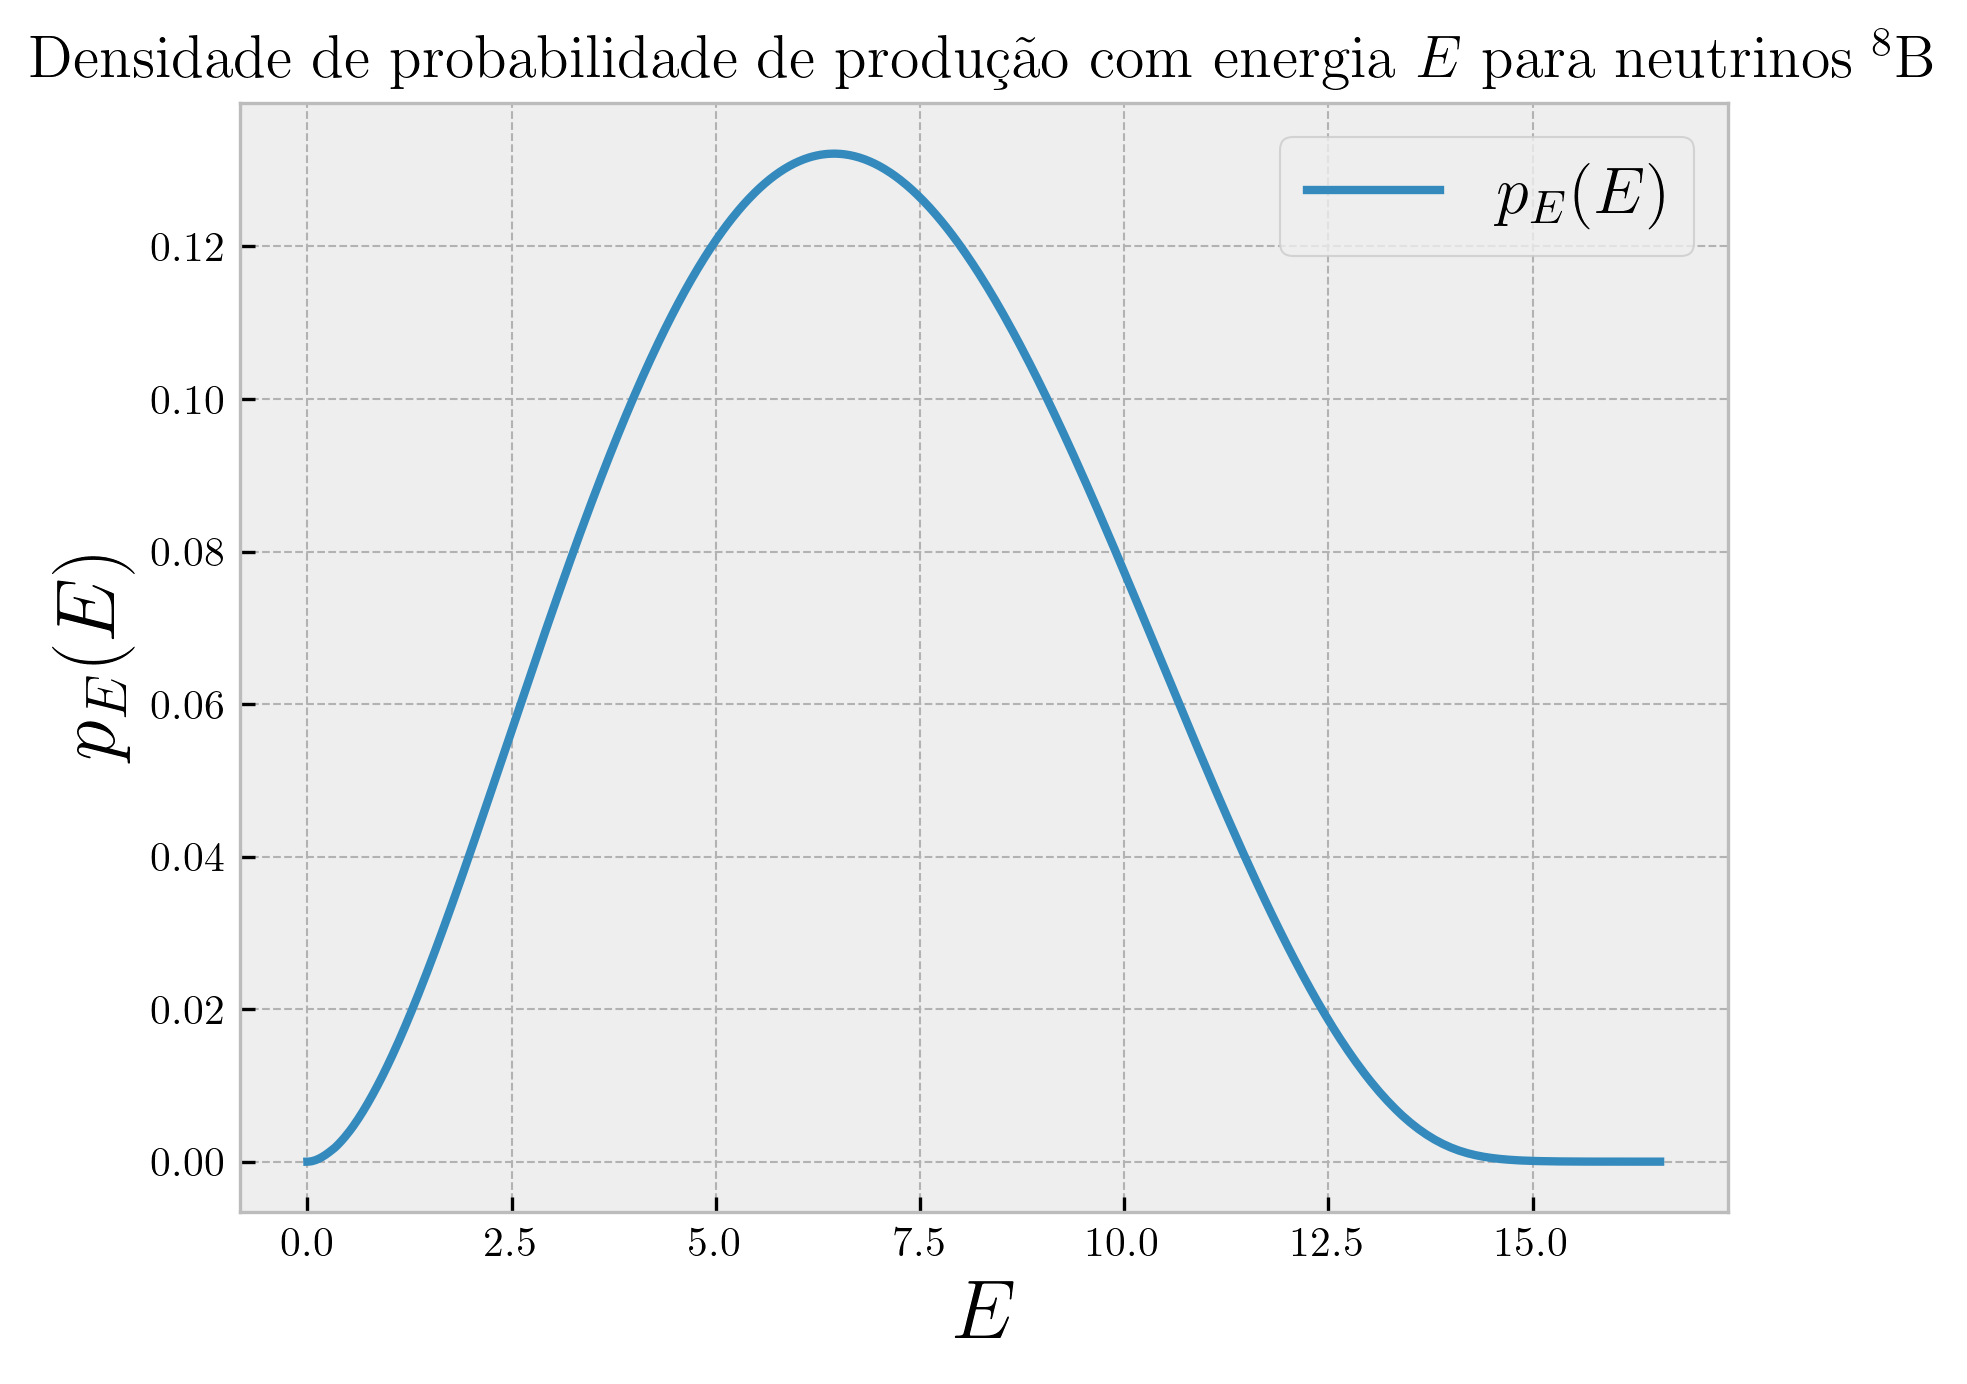
\includegraphics[width=.9\linewidth]{fig/nu8b-energy.png}
  \caption{}
  \label{fig:nu8b-energy}
\end{subfigure}%
\begin{subfigure}{.5\textwidth}
  \centering
  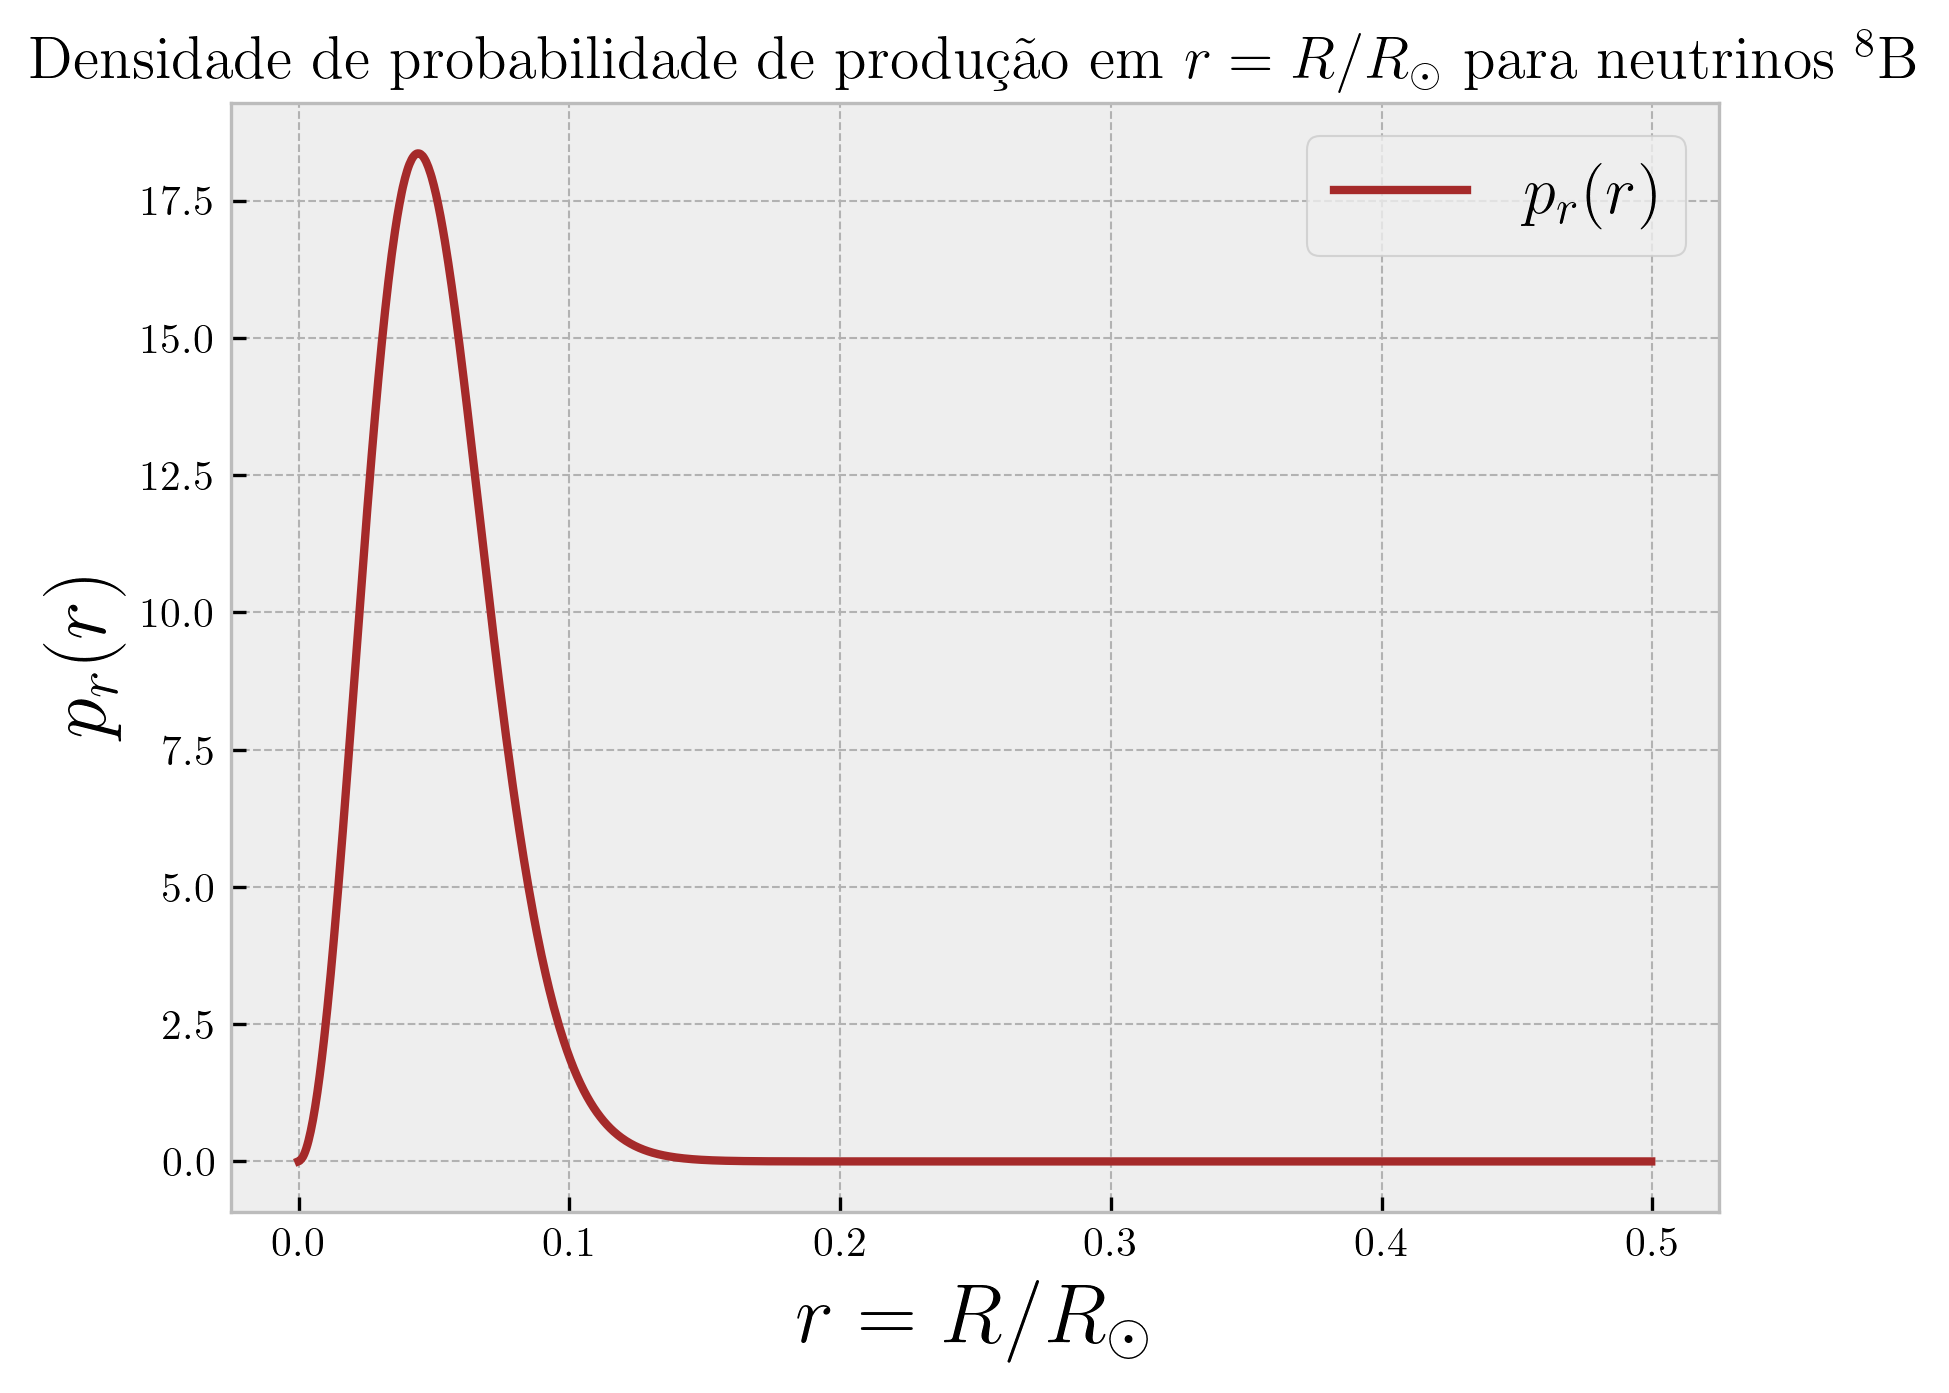
\includegraphics[width=.9\linewidth]{fig/nu8b-raio.png}
  \caption{}
  \label{fig:nu8b-raio}
\end{subfigure}
\caption{Distribuição de energia e raio dos neutrinos solares $^8\text{B}$.}
\label{fig:nu8b}
\end{figure}

Realizando o mesmo procedimento descrito no Apêndice \ref{sec:numeric}, podemos calcular numericamente a evolução para os neutrinos no interior do Sol. Somente consideraremos a condição inicial $\ket{\nu(0)} = \ket{\nu_e}$ devido aos neutrinos serem produzidos no estado do neutrino do elétron. Por enquanto, nos restringimos à condição de que eles são produzidos no centro do Sol e com a energia mais provável $E = 6.44 \unit{MeV}$ (vide Figura \ref{fig:nu8b-energy}), mas pretendemos utilizar as densidades de probabilidade das Figuras \ref{fig:nu8b-energy} e \ref{fig:nu8b-raio} com o fim de tirarmos médias no ponto de produção e obtermos também a probabilidade de sobrevivência $P(\nu_e \to \nu_e)$ em função da energia $E$ do neutrino do $^8$B.

Para dois sabores, a simulação numérica de oscilação no interior do Sol resulta na Figura \ref{fig:2nu-sol} a seguir:

\begin{figure}[H]
\centering
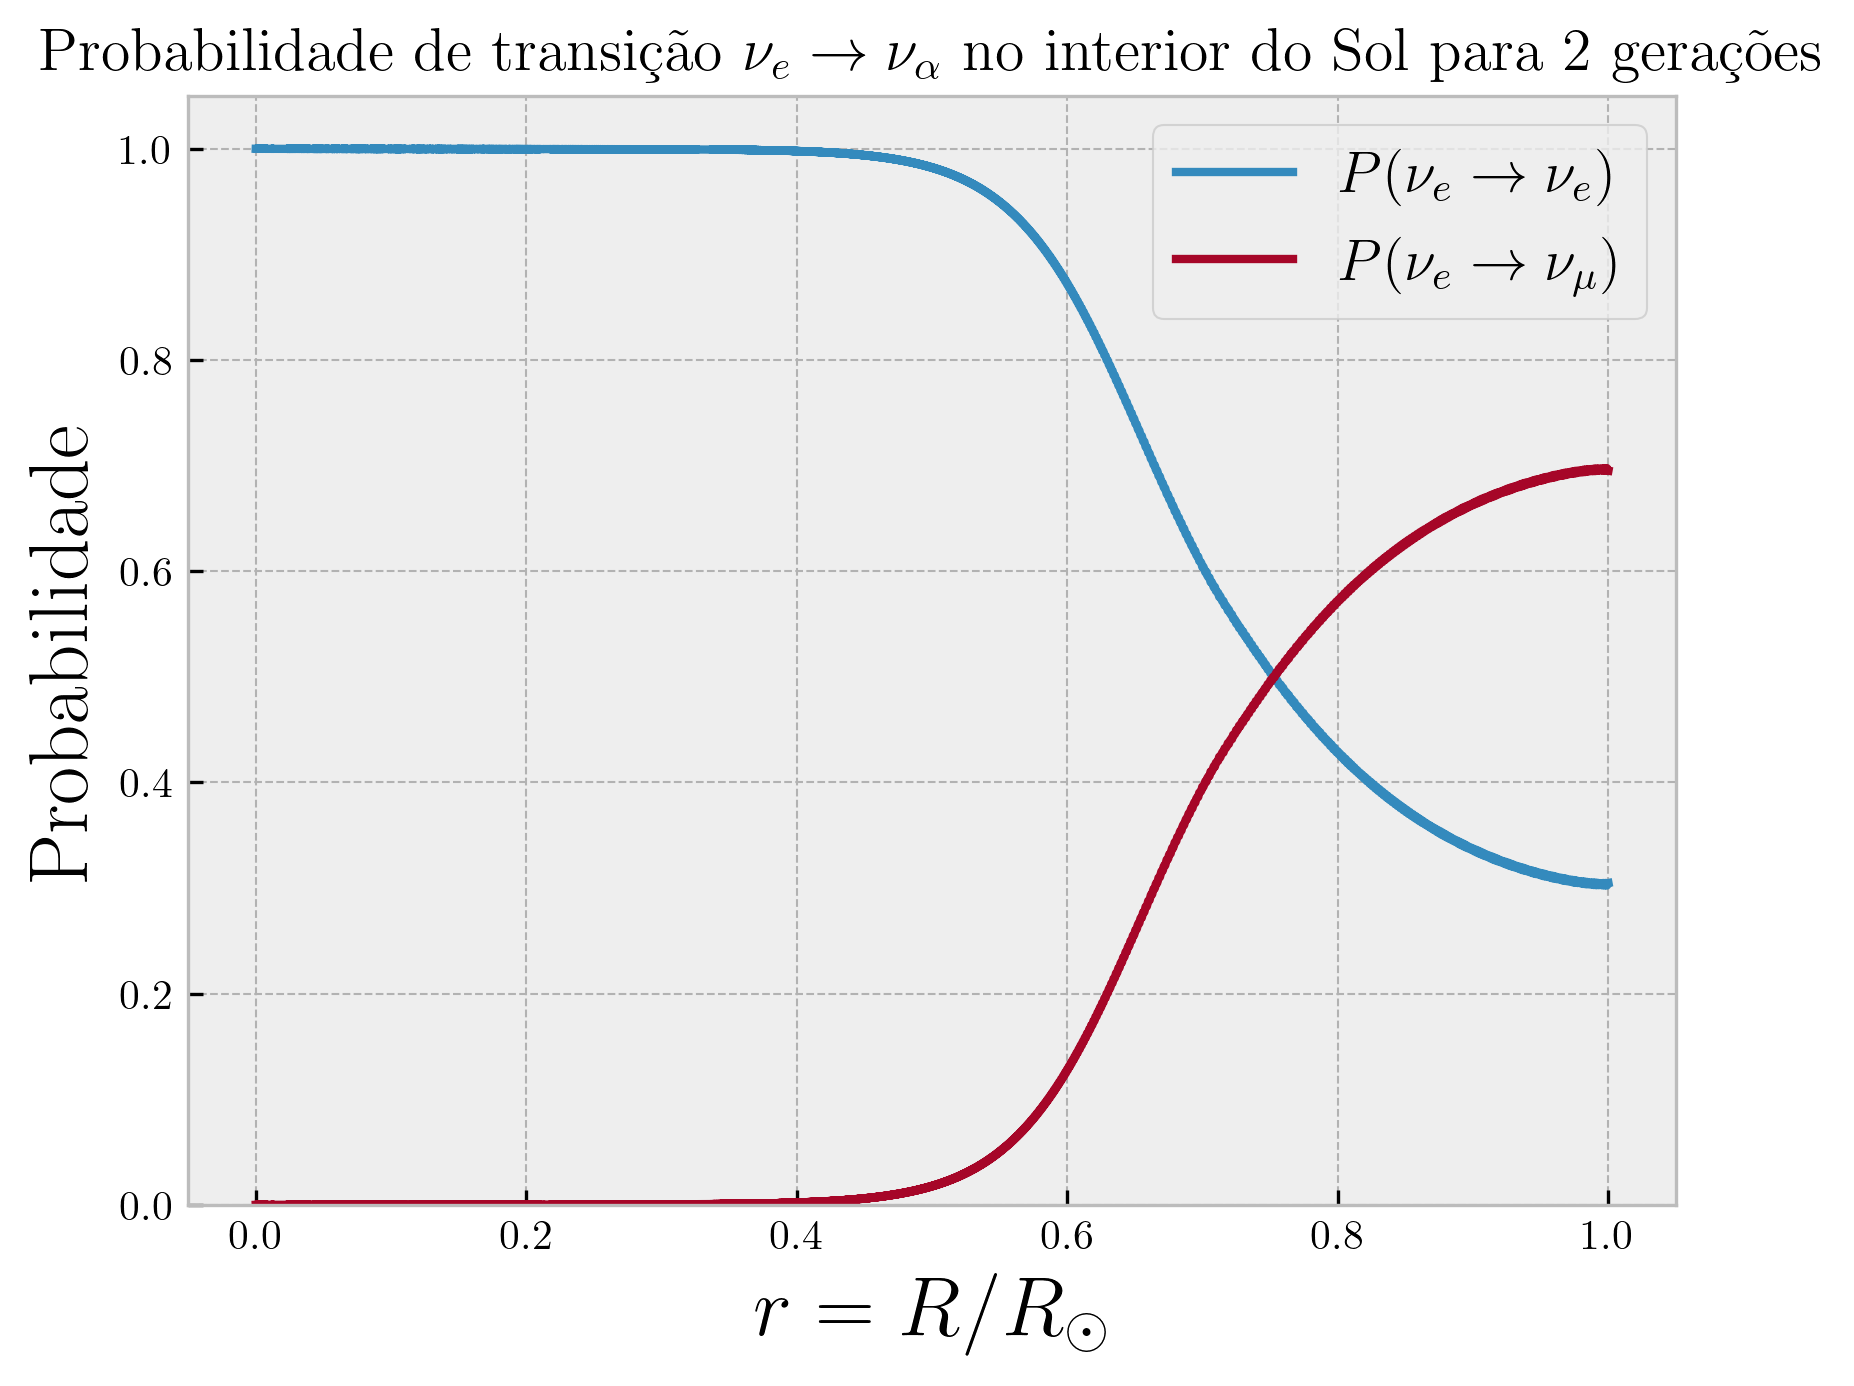
\includegraphics[width=0.65\textwidth]{fig/2nu-sol.png}
\caption{Oscilação de sabor no interior do Sol, com os parâmetros do NuFIT \cite{nufit} e dados do modelo solar BS2005 \cite{bahcall-model}, para duas gerações de neutrinos $\nu_e$ e $\nu_\mu$.}
\label{fig:2nu-sol}
\end{figure}

Vemos acima na Figura \ref{fig:2nu-sol} que, ao sair do Sol, a probabilidade $P(\nu_e \to \nu_e)$ se reduz a aproximadamente $0.3$, de maneira que seu comportamento não é mais oscilatório que nem no vácuo, Figura \ref{fig:2nu-vacuo}.

\begin{appendices}

\chapter{Abordagem numérica} \label{sec:numeric}

Qualquer equação de Schrödinger (com $\hbar = 1$) se escreve da forma
\begin{equation} \label{eq:schrodinger}
i \dv{\psi}{t}(t) = \H(t) \psi(t),
\end{equation}
onde, supondo que o problema seja $n$ dimensional, temos que $\psi = (\psi_1, \psi_2, \ldots, \psi_n)$ é um vetor complexo de $n$ componentes e $\H = (\H_{jk})_{n \times n}$ é uma matriz complexa $n \times n$.

Escrevendo a equação \ref{eq:schrodinger} em suas componentes $j$ e usando a decomposição cartesiana de números complexos $\psi_k = \eta_k + i \xi_k$ e $\H_{jk} = A_{jk} + i B_{jk}$, temos
$$
i \dv{\psi_j}{t} = \sum_k \H_{jk} \psi_k \implies i \dv{t}(\eta_j + i \xi_j) = \sum_k (A_{jk} + i B_{jk}) \, (\eta_k + i \xi_k)
$$
$$
\implies - \dv{\xi_j}{t} + i \dv{\eta_j}{t} =
\sum_k \big[ (A_{jk} \eta_k - B_{jk} \xi_k) +
i \, (B_{jk} \eta_k + A_{jk} \xi_k) \big] .
$$

Igualando partes real e imaginária, obtemos
\begin{equation} \label{eq:real-components}
\begin{cases}
\; \dv{\eta_j}{t} = \sum_k B_{jk} \eta_k  + \sum_k A_{jk} \xi_k; \\
\; \dv{\xi_j}{t}  = - \sum_k A_{jk} \eta_k  + \sum_k B_{jk} \xi_k.
\end{cases}
\end{equation}

Escrevendo \ref{eq:real-components} em forma matricial e identificando as partes reais $\eta = \Re\psi$, $A = \Re\H$ e imaginárias $\xi = \Im\psi$, $B = \Im\H$ do vetor $\psi$ e da matriz $\H$, obtemos
\begin{equation} \label{eq:real-matrix}
\dv{t}
\begin{pmatrix}
\Re \psi \\ \Im \psi
\end{pmatrix}
=
\begin{pmatrix}
\Im\H & \Re\H \\
-\Re\H & \Im\H
\end{pmatrix}
\begin{pmatrix}
\Re \psi \\ \Im \psi
\end{pmatrix},
\end{equation}
que deve ser entendida como uma equação envolvendo matrizes de matrizes.

A equação \ref{eq:real-matrix} está na forma ideal para ser resolvida por métodos numéricos usuais de EDO. Em nosso código em Python, aplicamos o método \texttt{DOP853} de Runge-Kutta ordem $8(5, 3)$ utilizando a biblioteca \texttt{scipy} \cite{scipy}.

\end{appendices}

\pagebreak

\chapter{Descrição e avaliação do Apoio Institucional recebido no período}\label{chp:apoioInst}

Durante o período correspondente a este relatório, o estudante não fez uso da reserva técnica.

\chapter{Participação em eventos científicos}\label{chp:particEvento}

O estudante compareceu em encontros de Journal Club do grupo de Física de Partículas do IFUSP, onde são discutidos semanalmente artigos publicados na área.

\chapter{Conclusões e Atividade Futuras}

Nas seções \ref{sec:2nu-vacuo} e \ref{sec:3nu-vacuo} retratamos o fenômeno de oscilação no vácuo e realizamos simulações numéricas com os parâmetros do NuFIT \cite{nufit}. Pretendemos ainda fazer uma comparação mais detalhada do que obtivemos com os resultados já consolidados na literatura.

Como foi descrito nas seções \ref{sec:weak-int} e \ref{sec:potencial-int}, o modelo de interação de Fermi que utilizamos consiste apenas em uma descrição efetiva da força fraca de corrente carregada, que sabemos ser explicada hoje pela teoria da interação eletrofraca. No próximo semestre pretendemos nos aprofundar no formalismo da Teoria Quântica de Campos, onde estudaremos em detalhe tópicos como Segunda Quantização, Matriz $S$ e diagramas de Feynman. Esperamos que isso nos possibilite compreender melhor como se dá a interação eletrofraca e o mecanismo de massa dos neutrinos.

Na seção \ref{sec:analise} apenas fizemos simulações numéricas para duas gerações com os neutrinos sendo produzidos no centro do Sol e somente consideramos sua energia mais provável. Pretendemos continuar essa análise, generalizando para três gerações e levando em conta as densidades de probabilidade do modelo solar BS2005 \cite{bahcall-model}, nas Figuras \ref{fig:nu8b-energy} e \ref{fig:nu8b-raio}. Com elas, temos como objetivo calcular, em função da energia $E$ com a qual o neutrino foi produzido, as médias no ponto de produção da probabilidade de sobrevivência $P(\nu_e \to \nu_e)$ no momento de saída do Sol. Nessas análises, consideraremos também o fluxo de neutrinos solares que chegam até a Terra e as seções de choque relevantes para que possamos comparar nossas simulações com os resultados de experimentos, como Super-Kamiokande e SNO.

Uma das dificuldades que surgiram durante nossas simulações numéricas foi o tempo necessário para o algoritmo finalizar. Suspeitamos que a razão disso seja porque os parâmetros de nossa EDO \ref{eq:real-matrix} façam com que ela se caracterize com uma \textit{stiff equation}. Para lidar com este problema, pretendemos nos aprofundar no artigo \cite{efficient-nu}, que propõe um método alternativo de integração de EDOs envolvendo neutrinos, o qual podemos aproveitar para otimizar o tempo de nossas simulações.


%%-----
%% Referências bibliográficas
%%-----
\addcontentsline{toc}{chapter}{\bibname}
%\bibliographystyle{abntex2-num}
\bibliography{bibliografia}
\bibliographystyle{ieeetr}

%%-----
%% Fim do documento
%%-----
\end{document}
